\section{Results}

    To evaluate the 95$\%$ confidence level (CL) limits on the new physics production cross section, an asymptotic CL$_{S}$ method~\cite{cls,cls1} is used where the systematic uncertainties in the signal and background predictions are treated as nuisance parameters with log-normal prior distributions. %Nuisances arising from uncertainties are applied for the normalization of signal and background processes. 

%%---------Model Independent limits
\subsection{Model-independent limits}

  Due to the variety of signals which can contribute to this final state, we present results for a generic signal using the model-independent selection described in Section~\ref{sec:event_selection}. Although this selection does not have as strong of discrimination power between signal like and background like events compared to the misreconstructed \met rejection selections, it does have less model dependence. This is due to \met significance and $\tilde{\met}$ minimization requirements having a non trivial efficiency dependence on the underlying event and observed \met.

  The total expected SM background and observed data events after the model-independent selection are found to be compatible within the systematic uncertainties. Table~\ref{table:modelInd} shows a comparison of the event yields estimated for background processes and the observed data. Figure~\ref{fig:modelInd} shows the $M_{T}$ and \met distributions after the model-independent selection has been applied.


\begin{table}[H]                                                                  
\center    
{          
\begin{tabular}{|c|c|}                                                             
\hline     
Process & \# of Events \\                                                              
\hline     
$\gamma +$ jets                          & $(313 \pm 50 ) \times 10^3$ \\
${\rm jet}\rightarrow \gamma$        & $(906 \pm 317 ) \times 10^2$ \\
${\rm e} \rightarrow \gamma$         & $(1035 \pm 62 ) \times 10^1$ \\
$W(\to \ell\nu)+\gamma $                 &  $2239 \pm 111$ \\
$Z( \to \nu \bar{\nu} )+\gamma    $      &  $2050 \pm 102$ \\
Other                                    &  $1809 \pm 91$ \\
\hline
Total background                       &   $(420 \pm 82 ) \times 10^3$ \\
\hline
Data                                   &  $442 \times 10^3$  \\
\hline     
\end{tabular}  
\caption{Comparison of event yields for observed data and background, after the model-independent selection.}
\label{table:modelInd}
}          
\end{table}

  %% figure of ModInd spectrun selection 
\begin{figure}[H]                  
\centering   
%{\label{fig:QCDPt}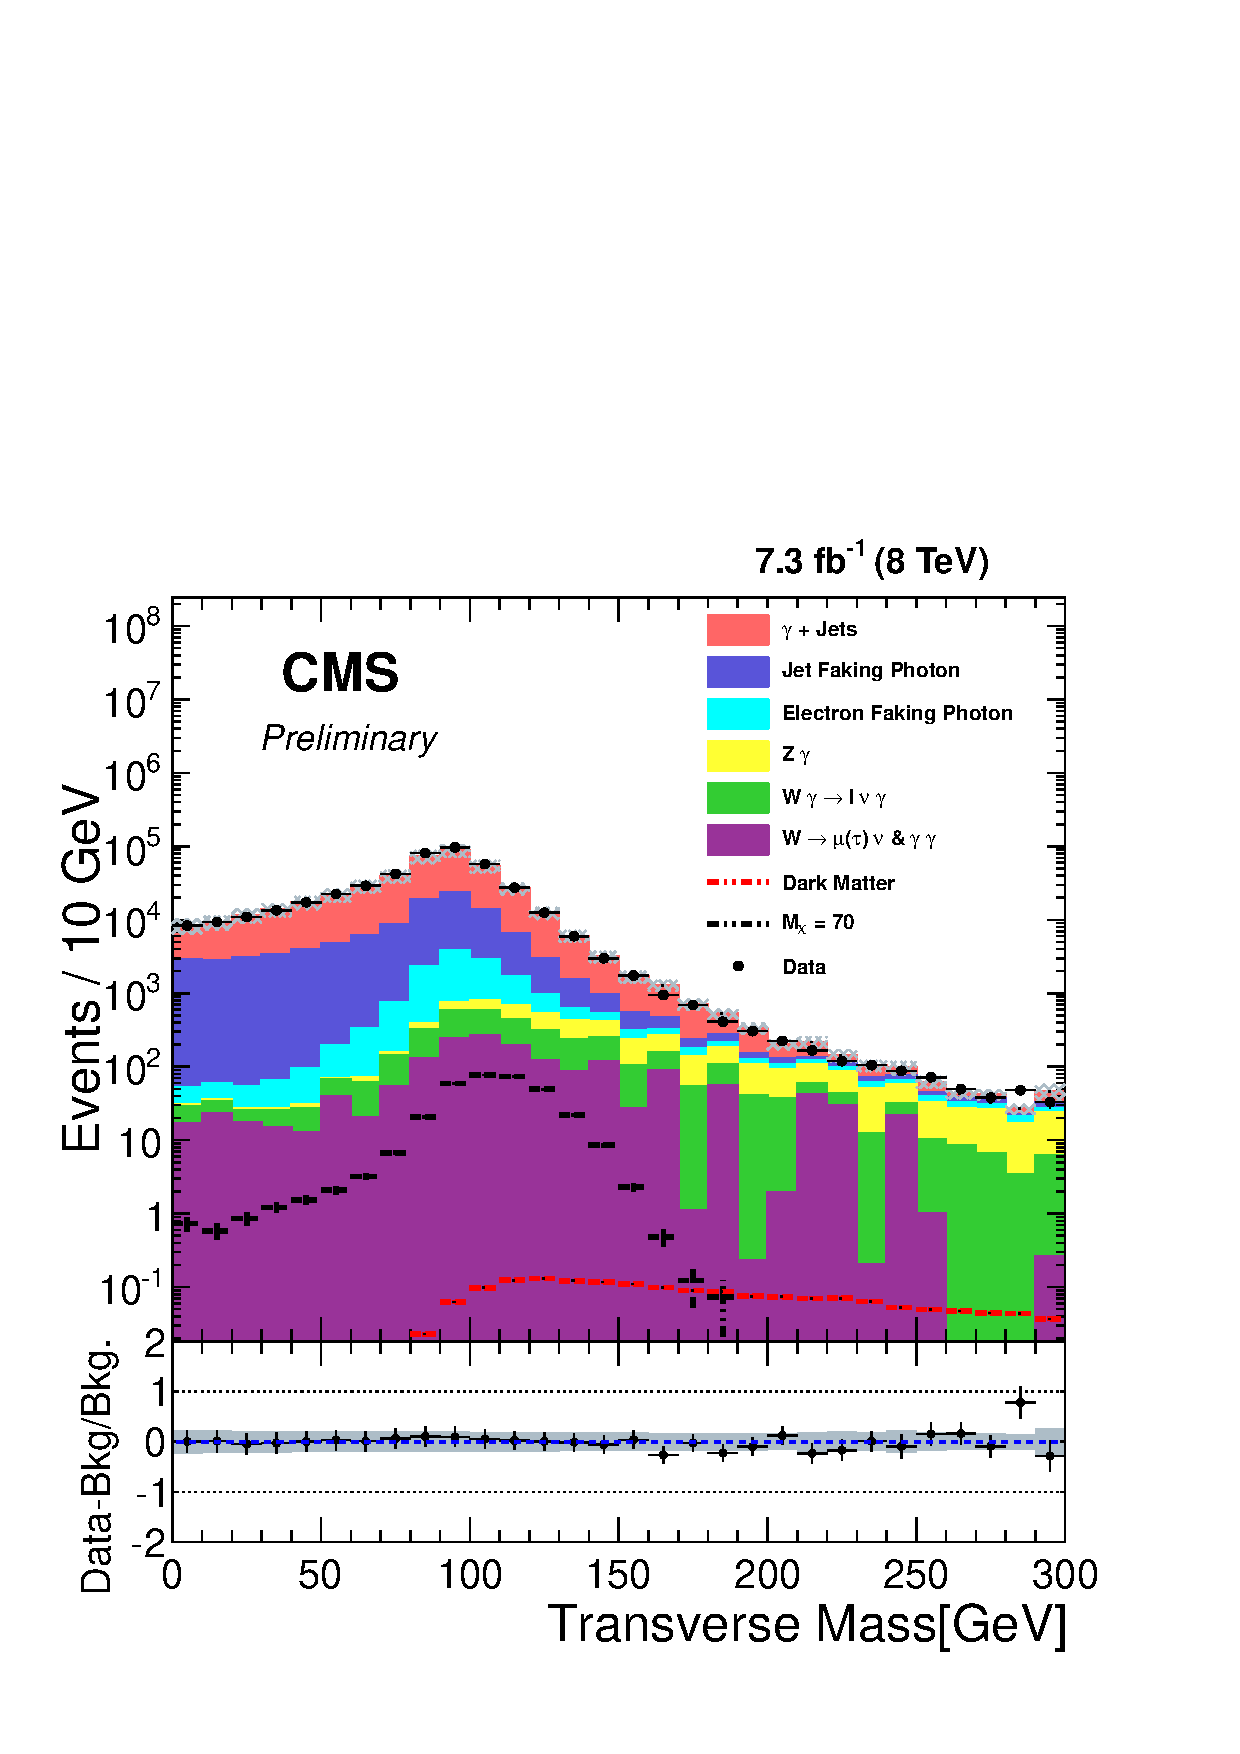
\includegraphics[scale=0.4]{Unblinding/ModelIndep/StackedHisto_MT.pdf}}                           
%{\label{fig:QCDMET}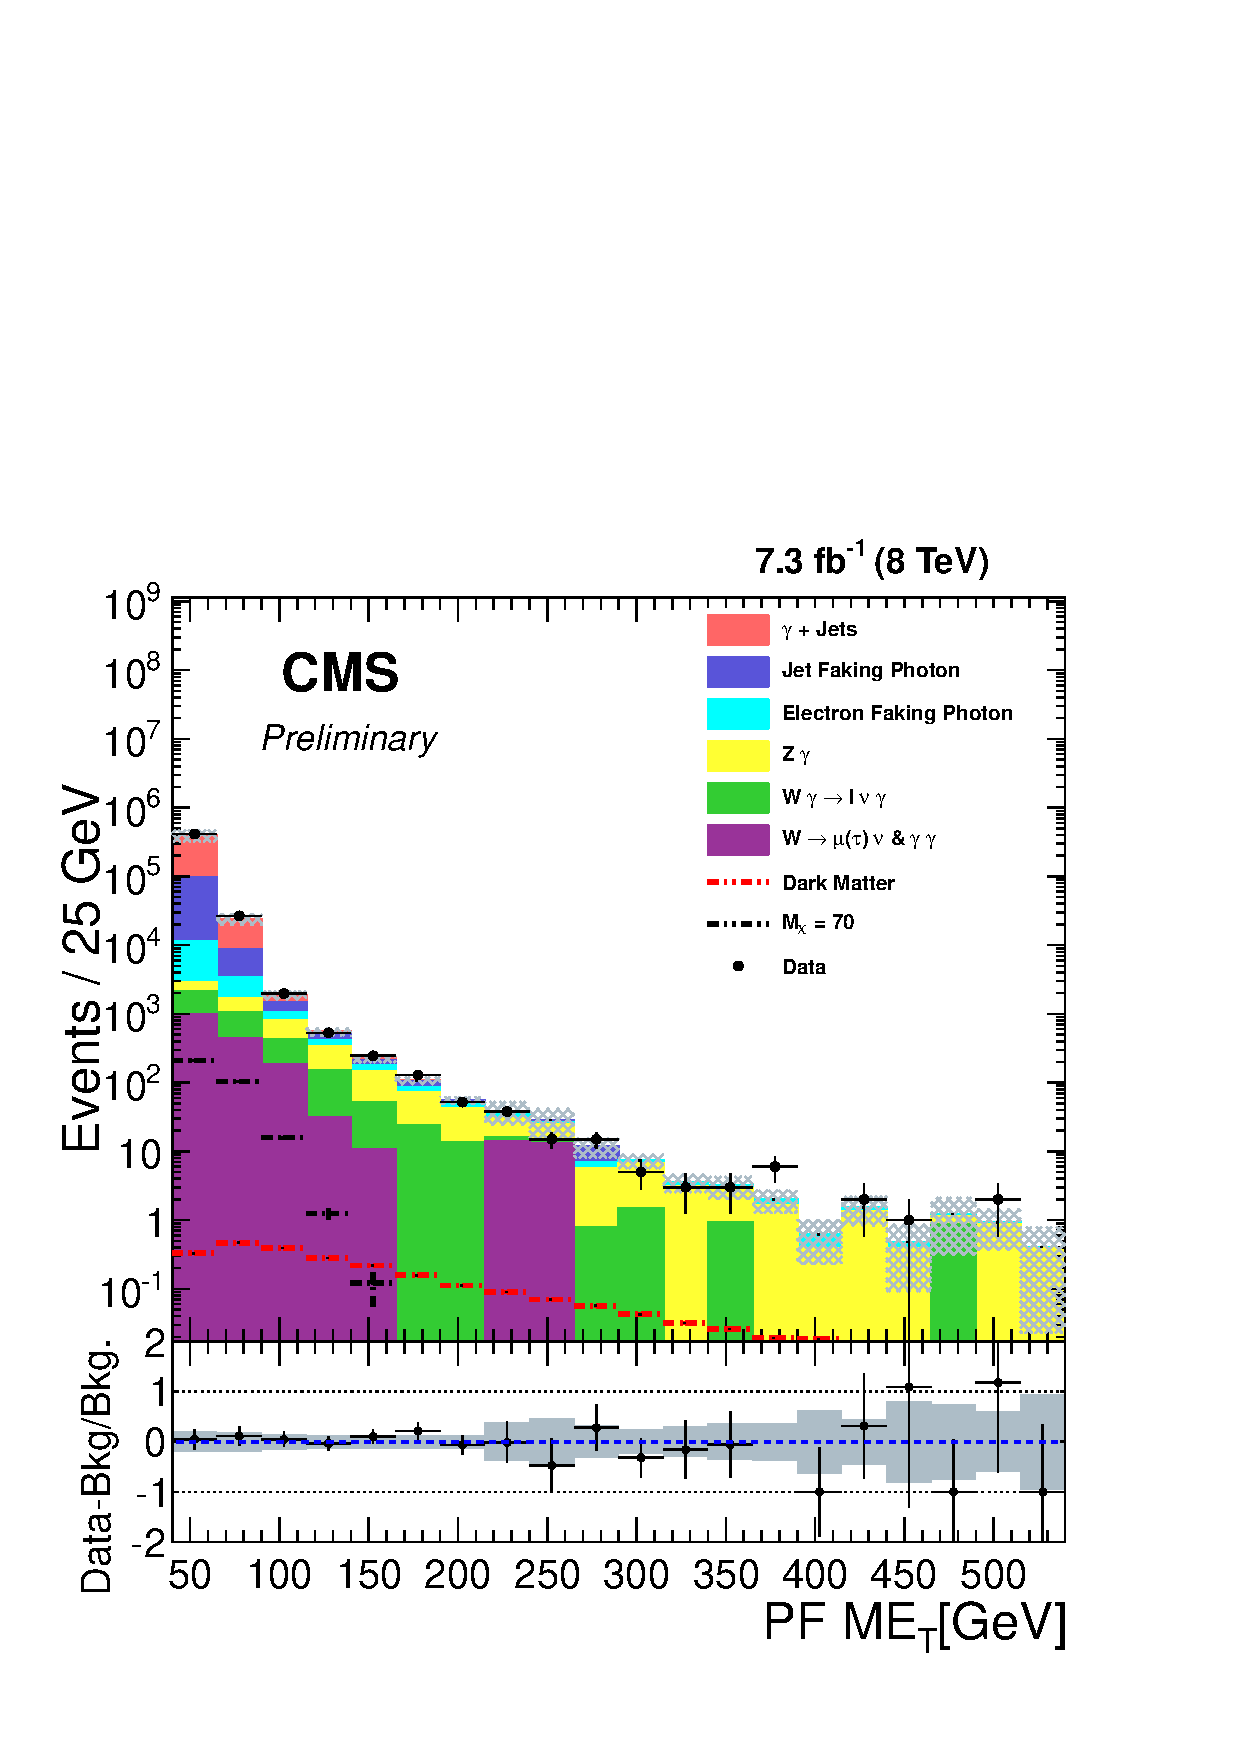
\includegraphics[scale=0.4]{Unblinding/ModelIndep/StackedHisto_MET.pdf}}                         
{\label{fig:QCDPt}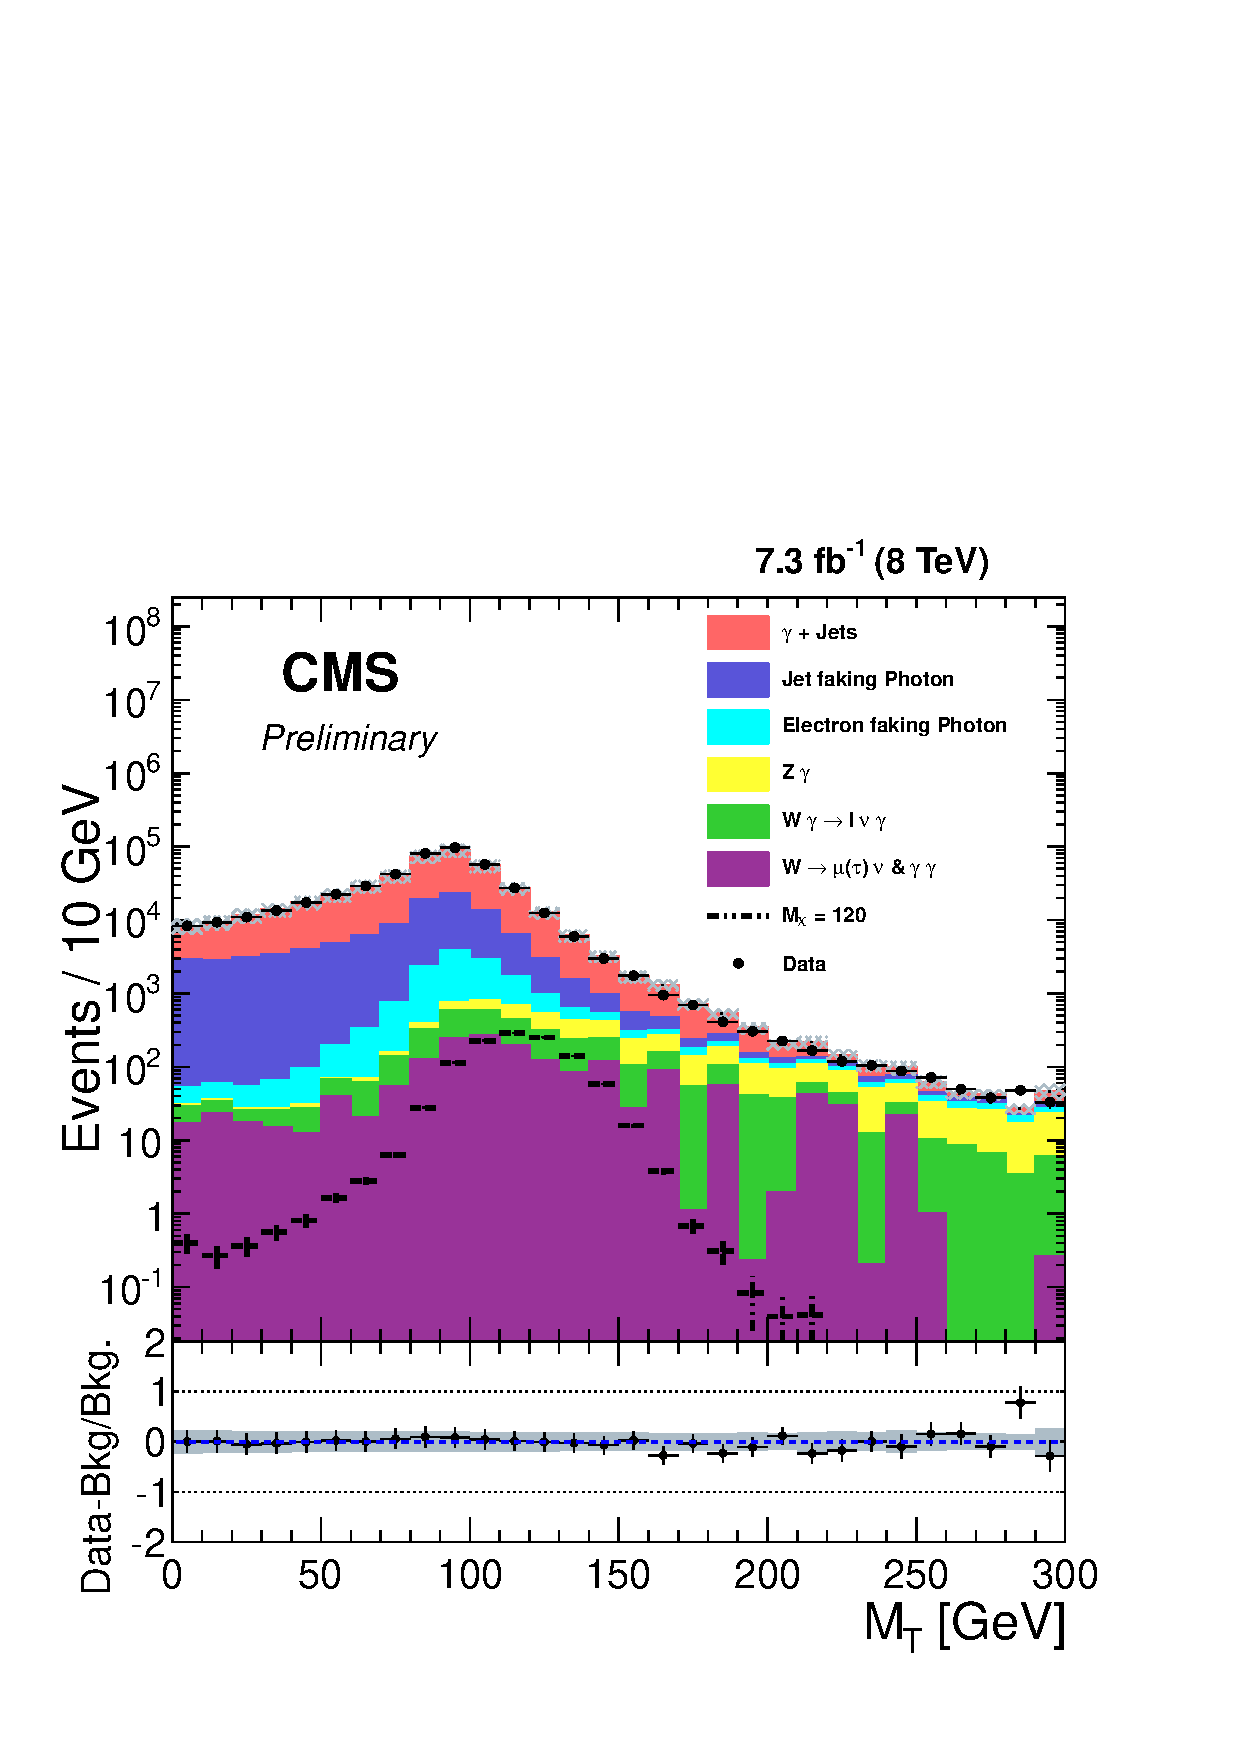
\includegraphics[width=0.45\textwidth]{PAS_Plots2/StackedHisto_MT.pdf}}                           
{\label{fig:QCDMET}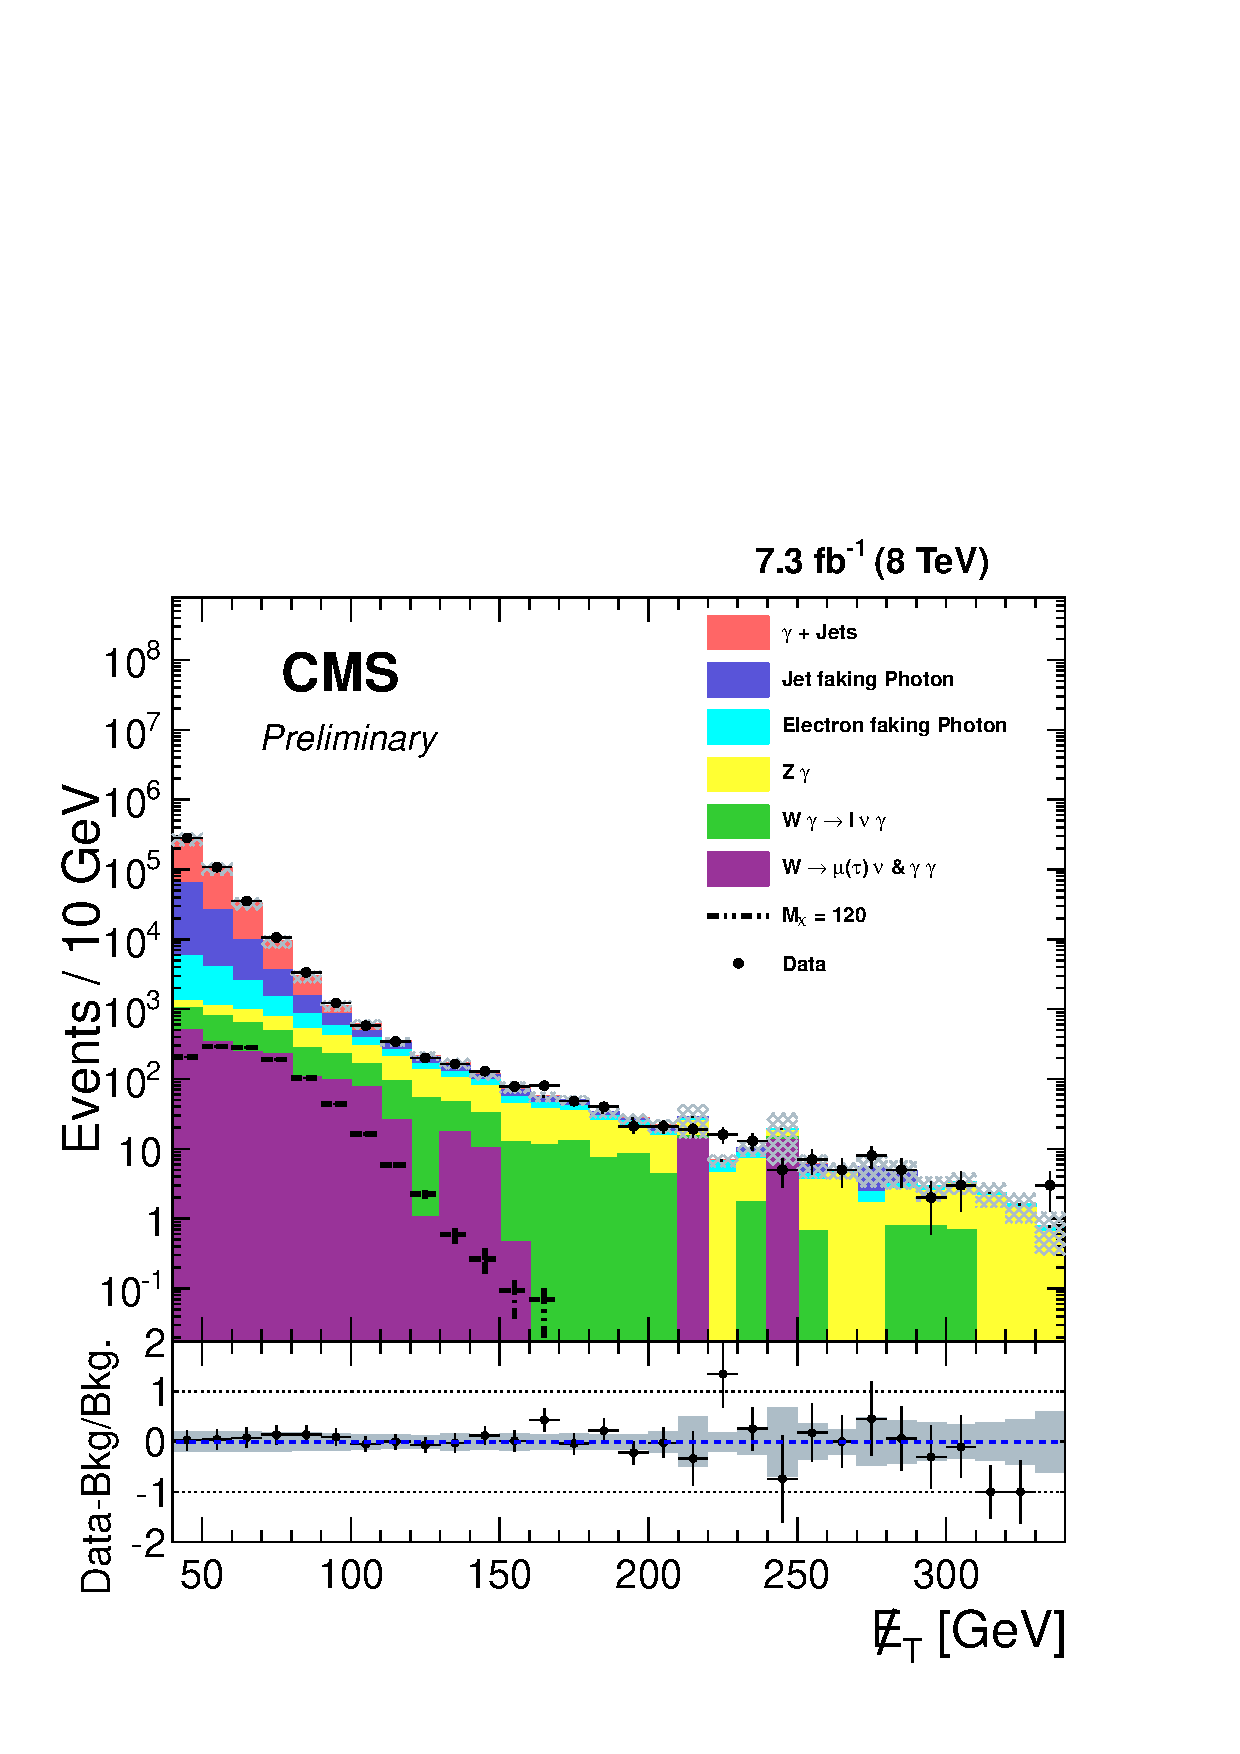
\includegraphics[width=0.45\textwidth]{PAS_Plots2/StackedHisto_MET.pdf}}                         
\caption{The $M_{T}$ and \met distributions for data, background estimates, and signal after the model-independent selection. The bottom panels in each plot show the ratio of (data - background)/background and the gray band includes both the statistical and systematic uncertainty on the background prediction. }                           
\label{fig:modelInd}                     
\end{figure} 

  Figure~\ref{fig:limit_MI} shows the observed and expected model-independent $95\%$ CL upper limits on $\sigma\times BR\times A\times\epsilon$ for different \met and $M_{T}$ thresholds. The observed and expected limits are also shown in Fig~\ref{fig:limit_MI}(c) at a 95$\%$ CL for $M_{T}> 100$ GeV and as a function of \met.


\begin{figure}[H]        
\centering                
{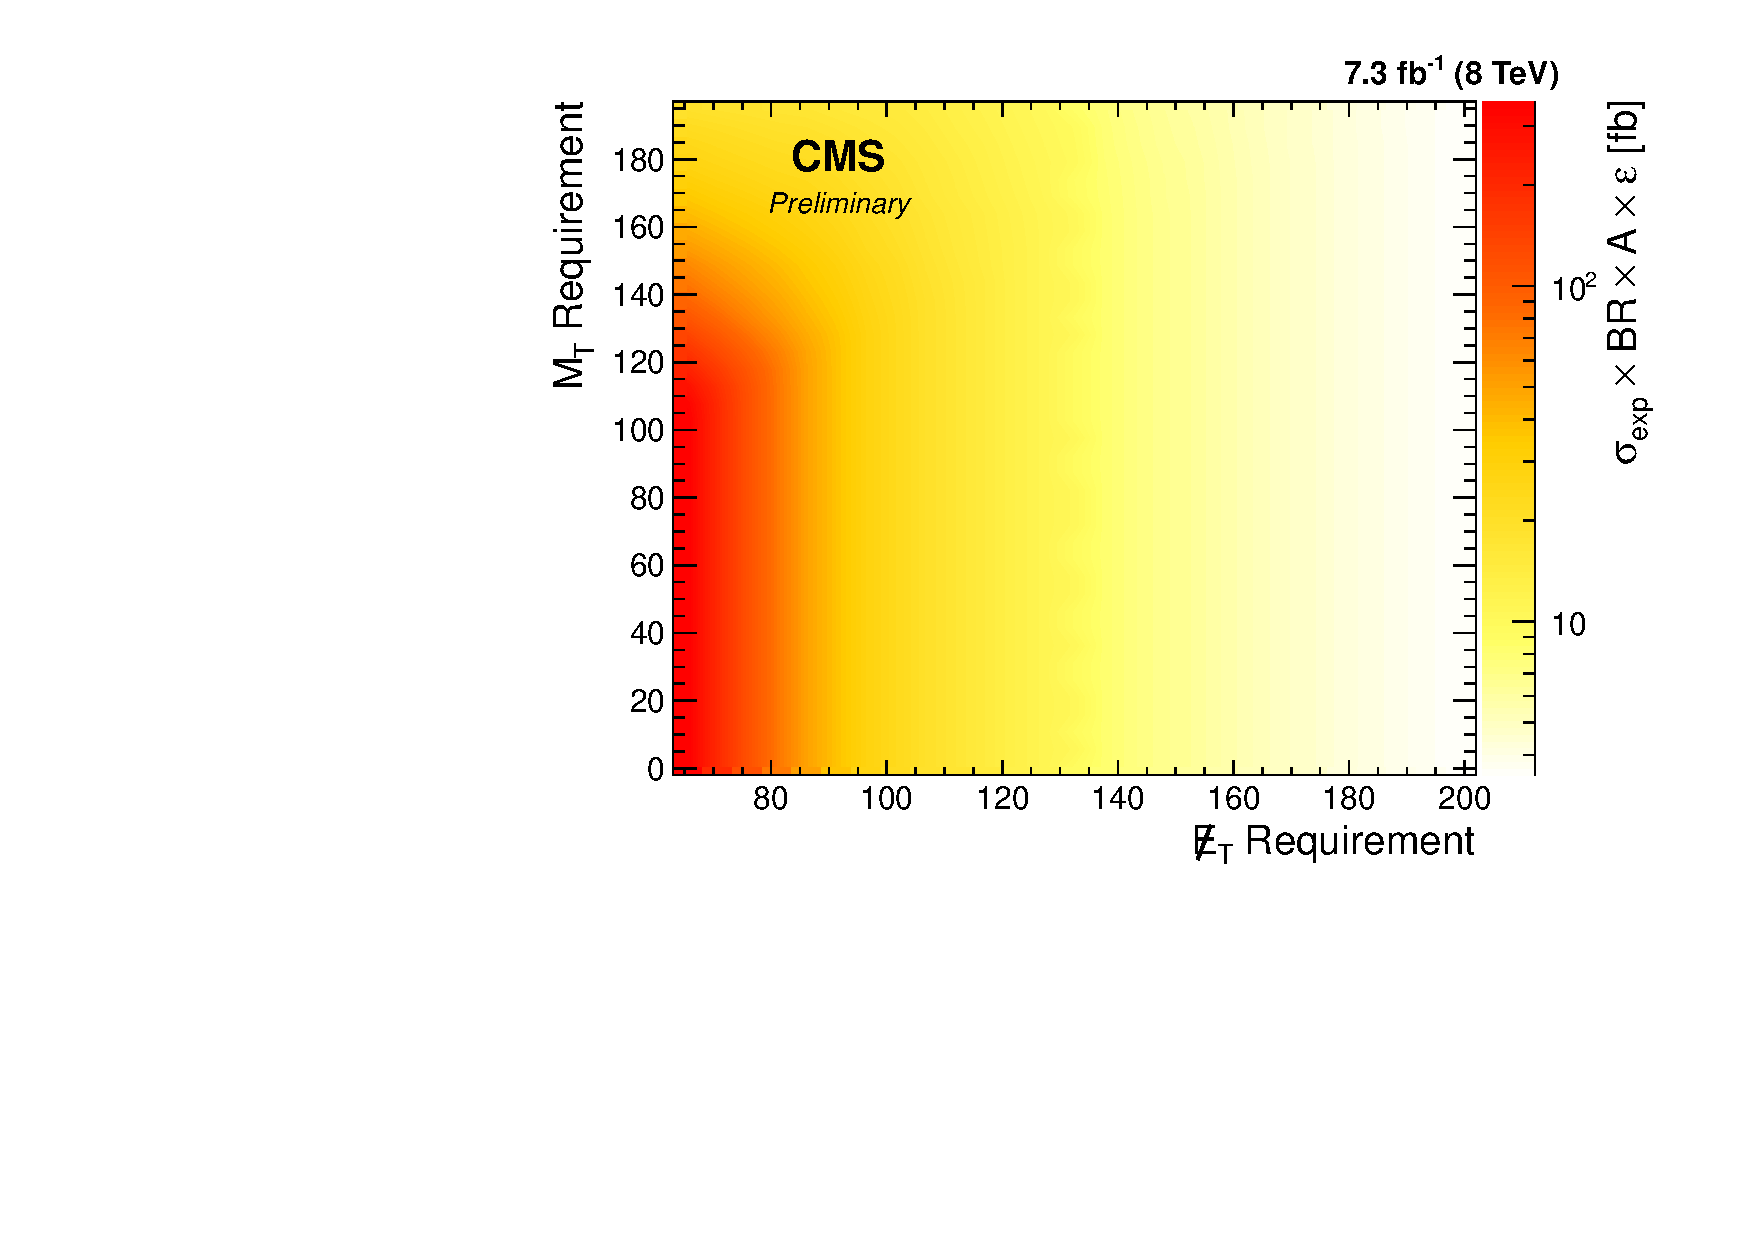
\includegraphics[width=0.45\textwidth]{PAS_Plots/pretty/2d_expected.pdf}}
{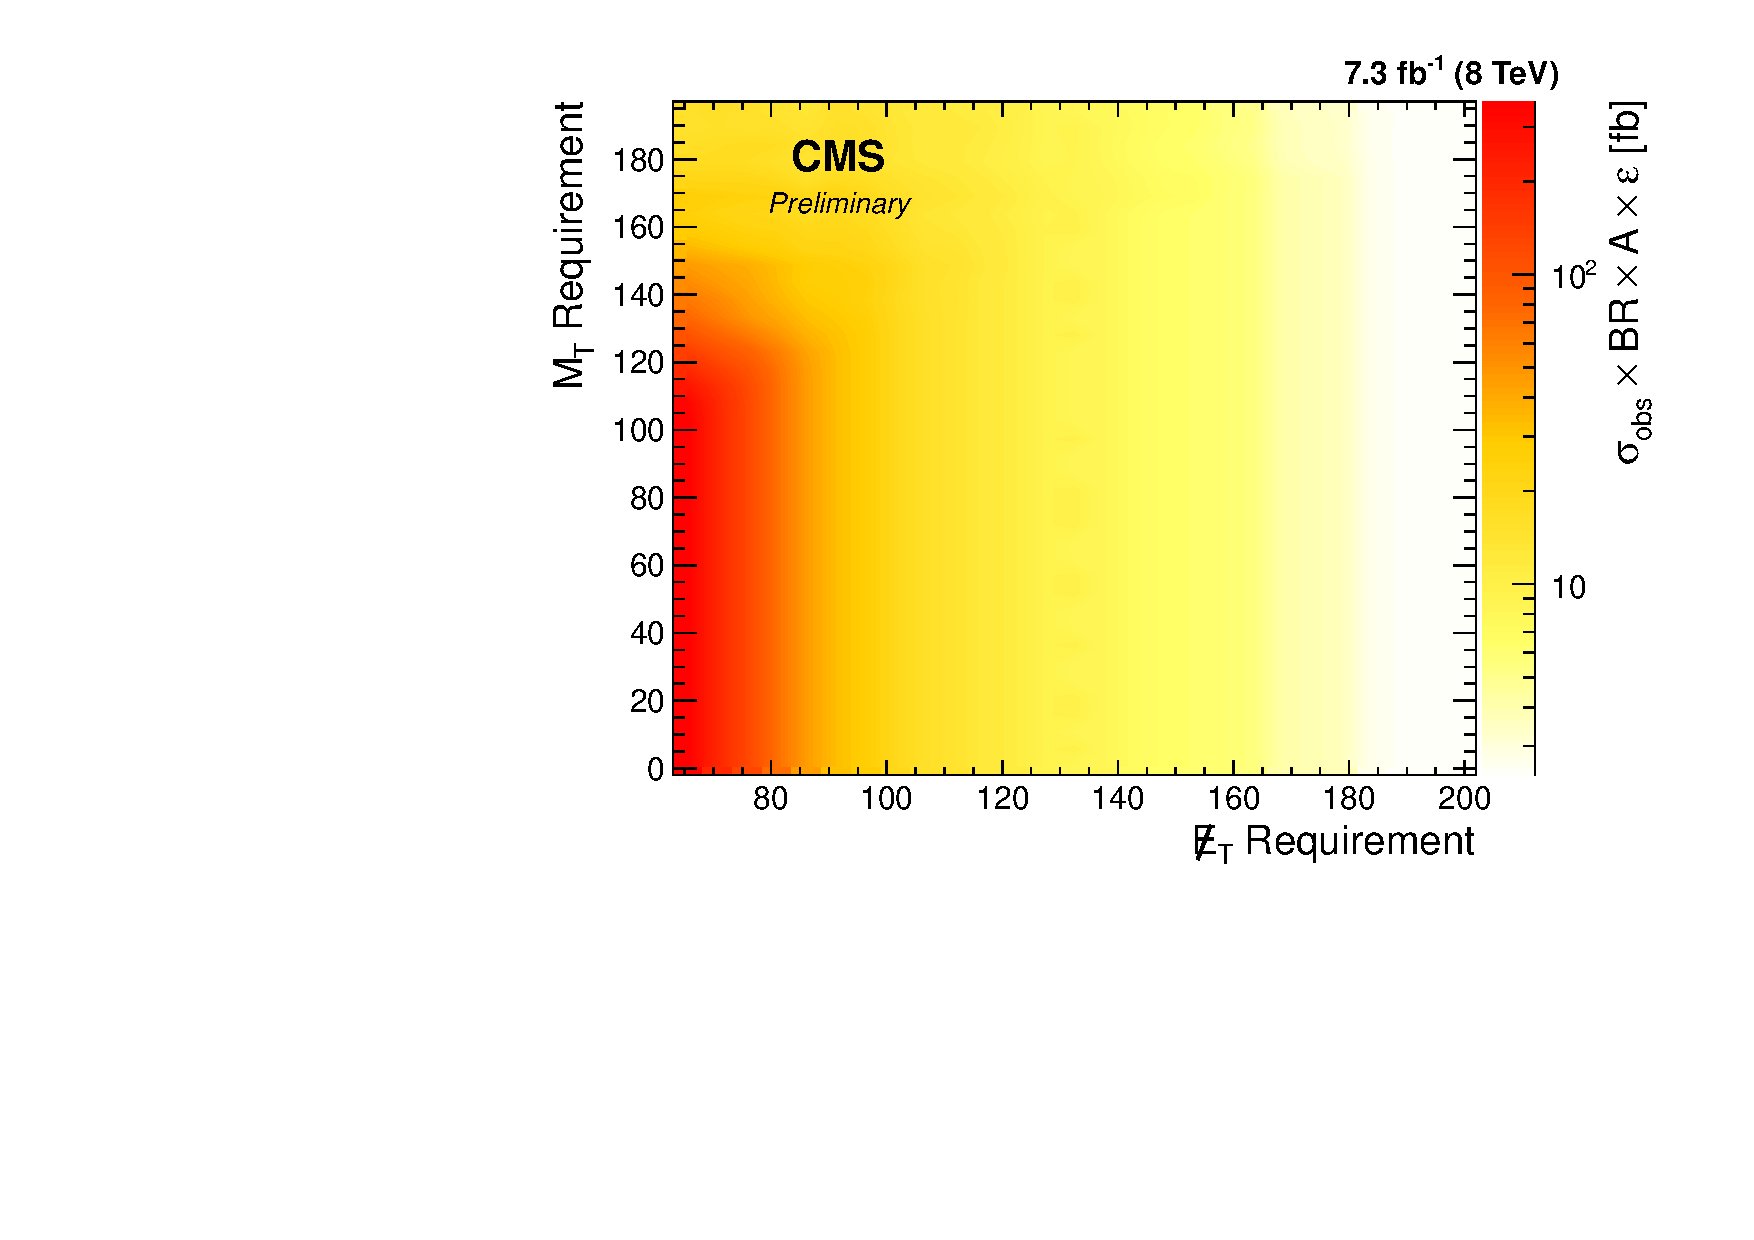
\includegraphics[width=0.45\textwidth]{PAS_Plots/pretty/2d_observed.pdf}} \\
{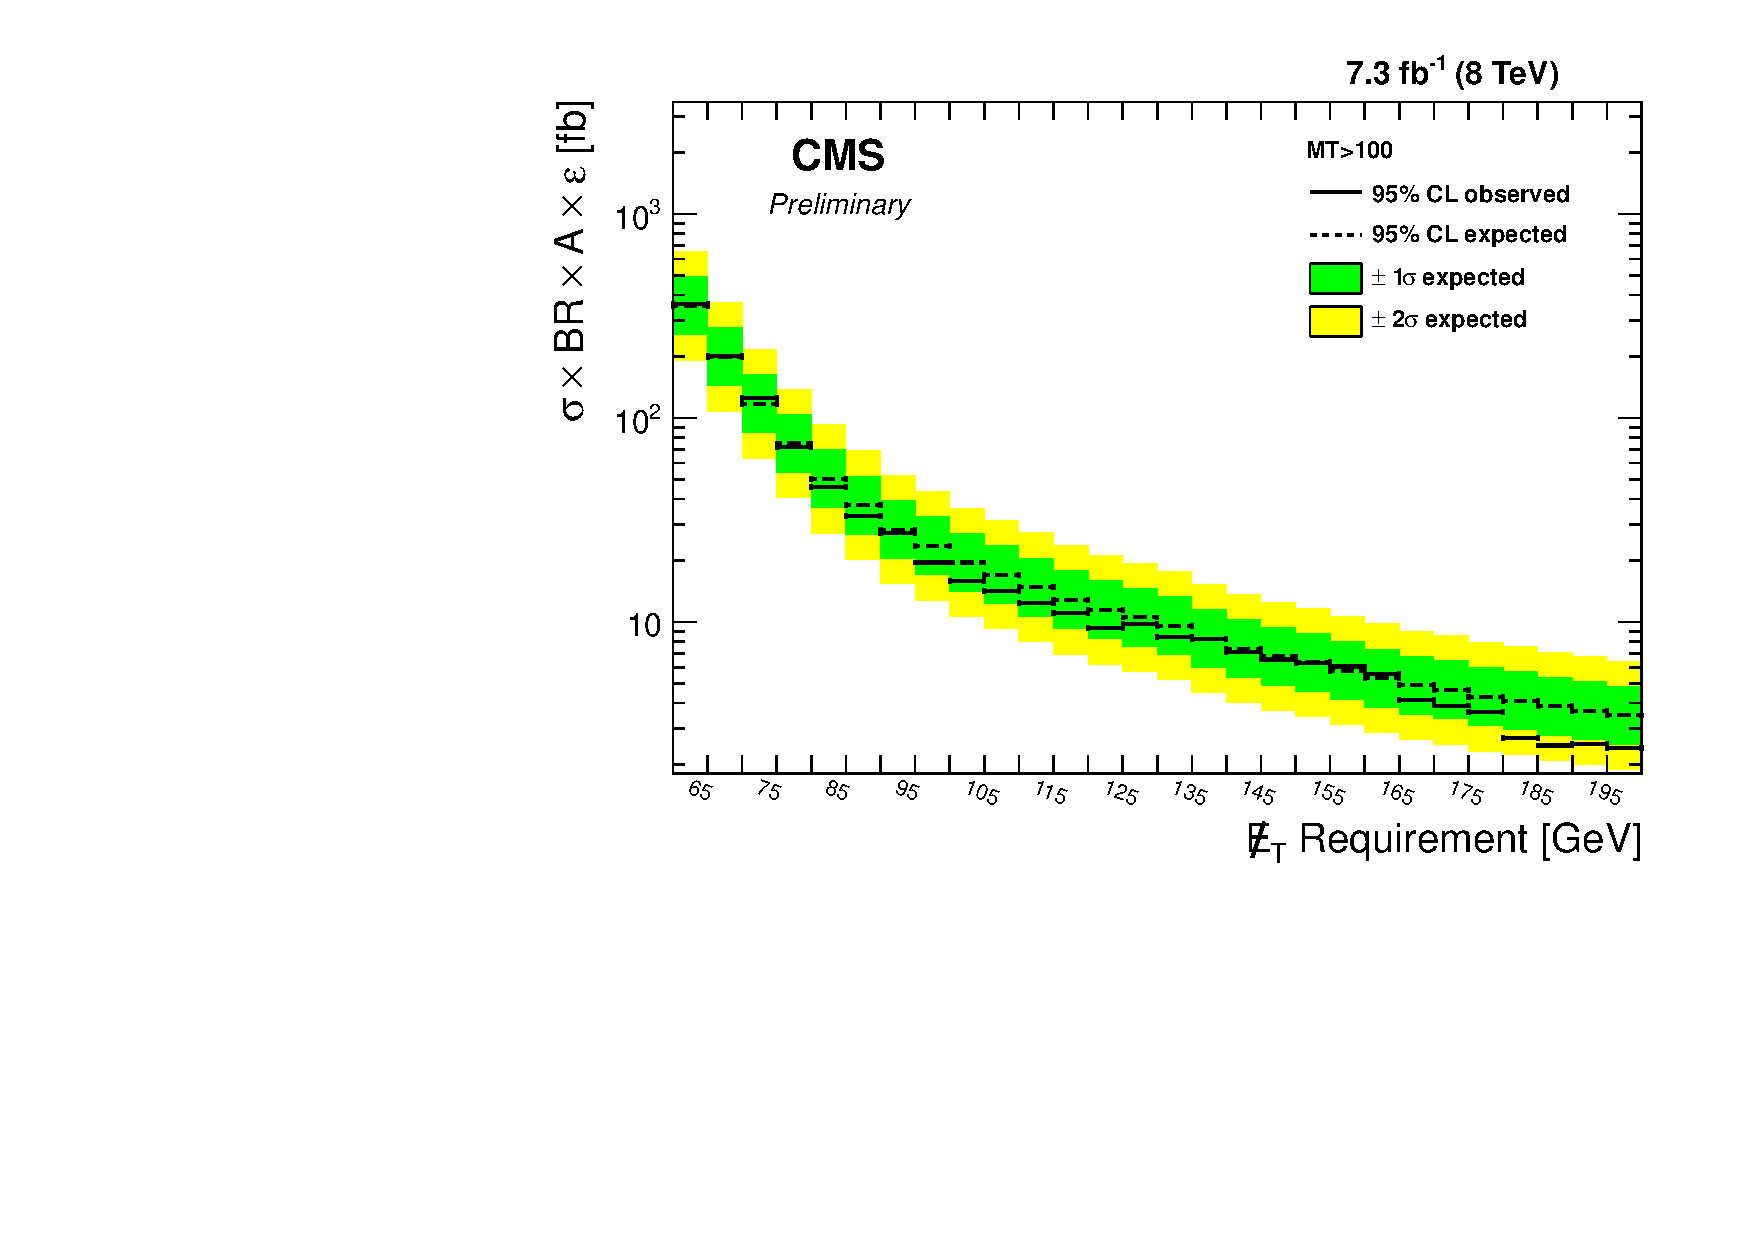
\includegraphics[width=0.45\textwidth]{PAS_Plots/LimitPlotVsMET_MT100.pdf}}
%{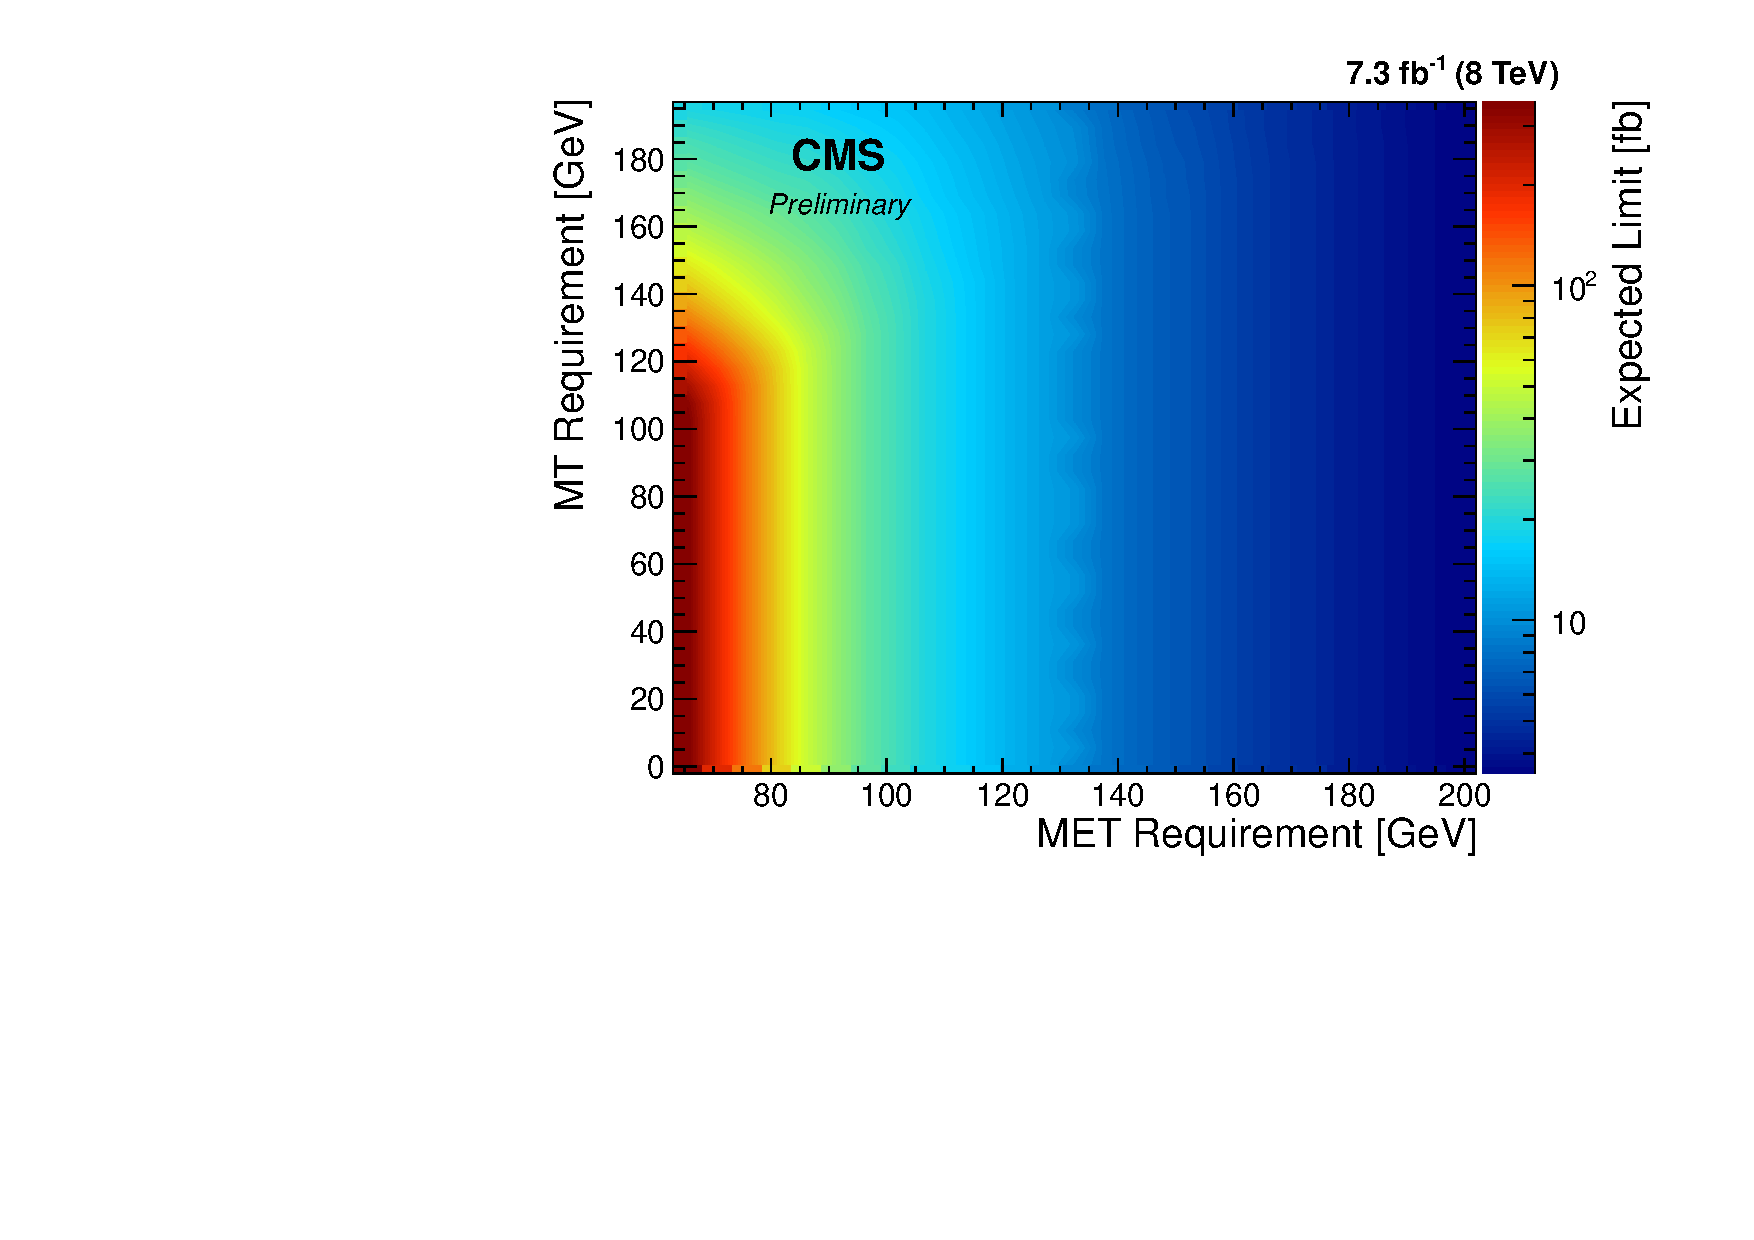
\includegraphics[scale=0.4]{Unblinding/ModelIndep/2d_final_expected.pdf}}
%{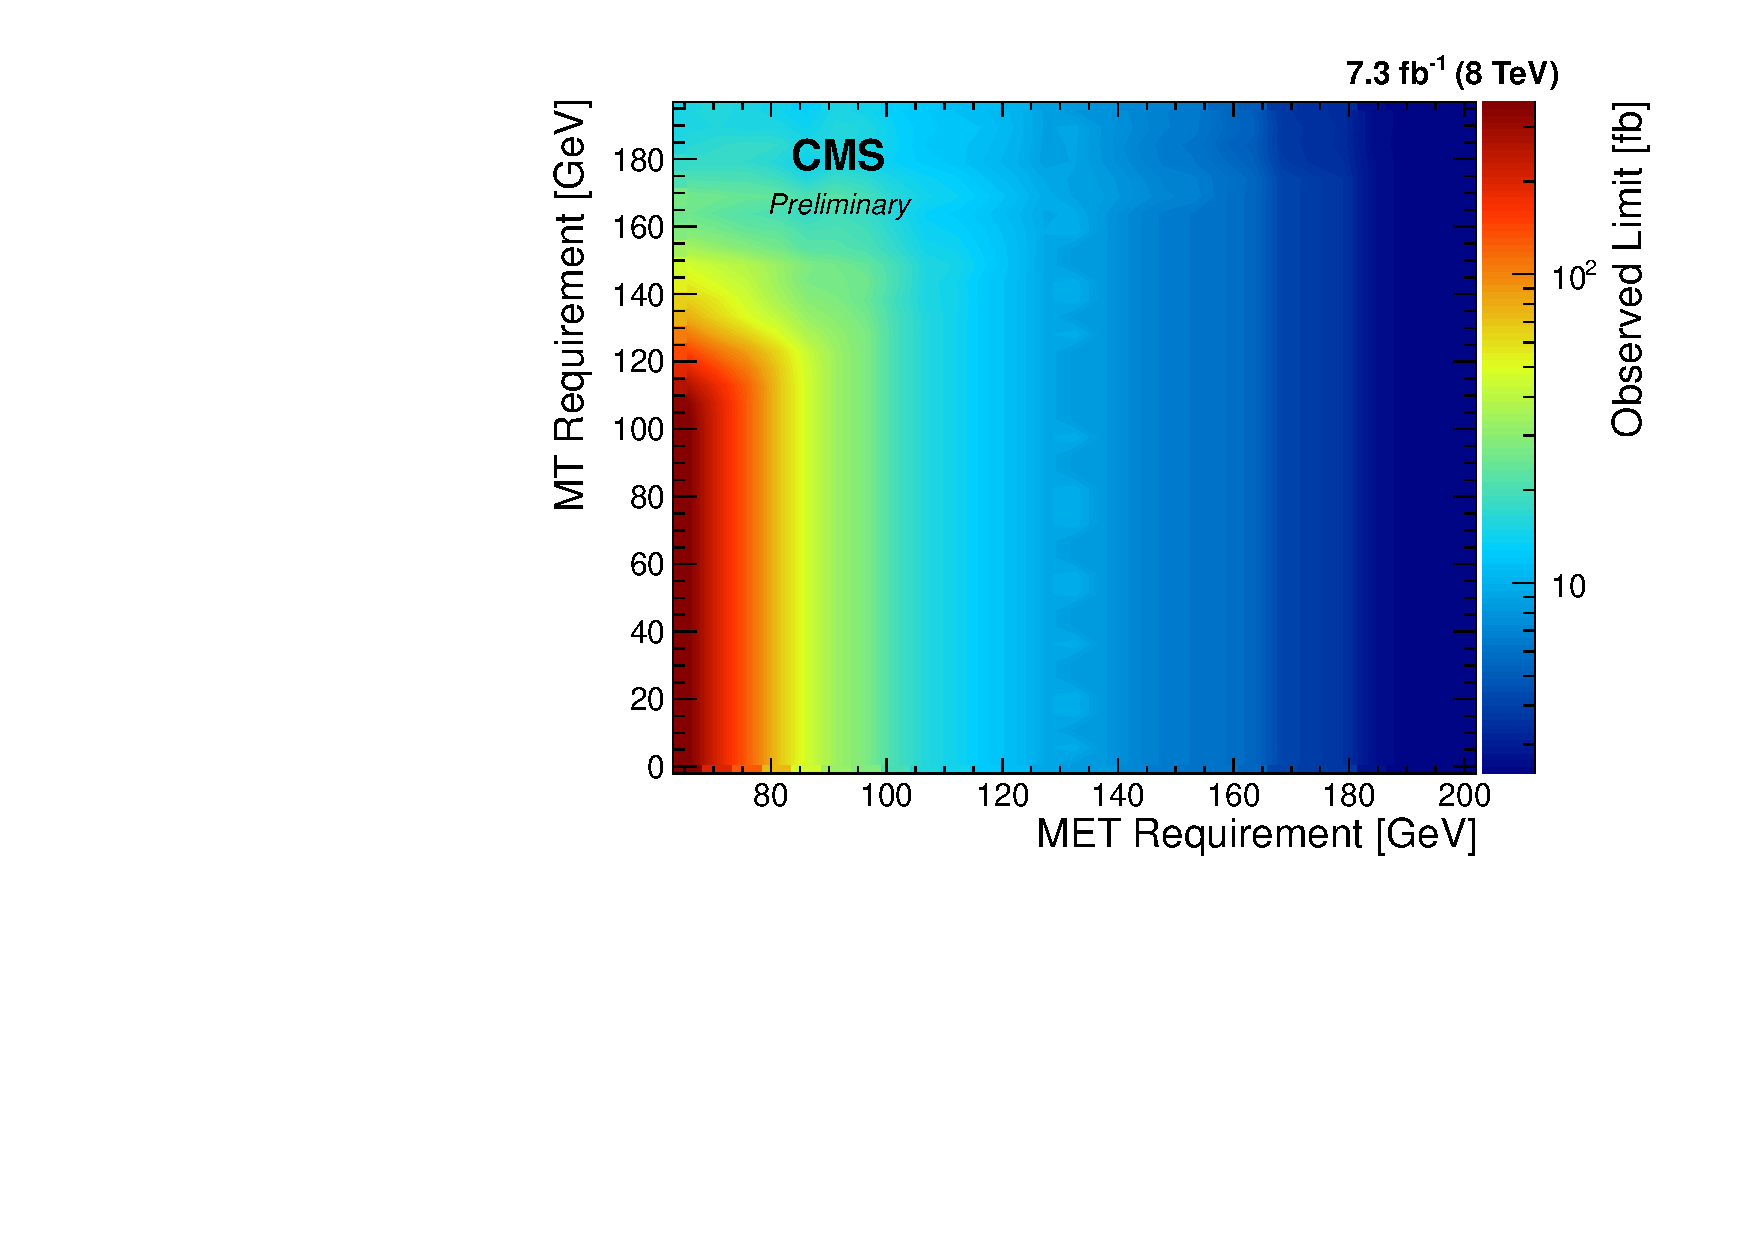
\includegraphics[scale=0.4]{Unblinding/ModelIndep/2d_final_observed.pdf}} \\
%{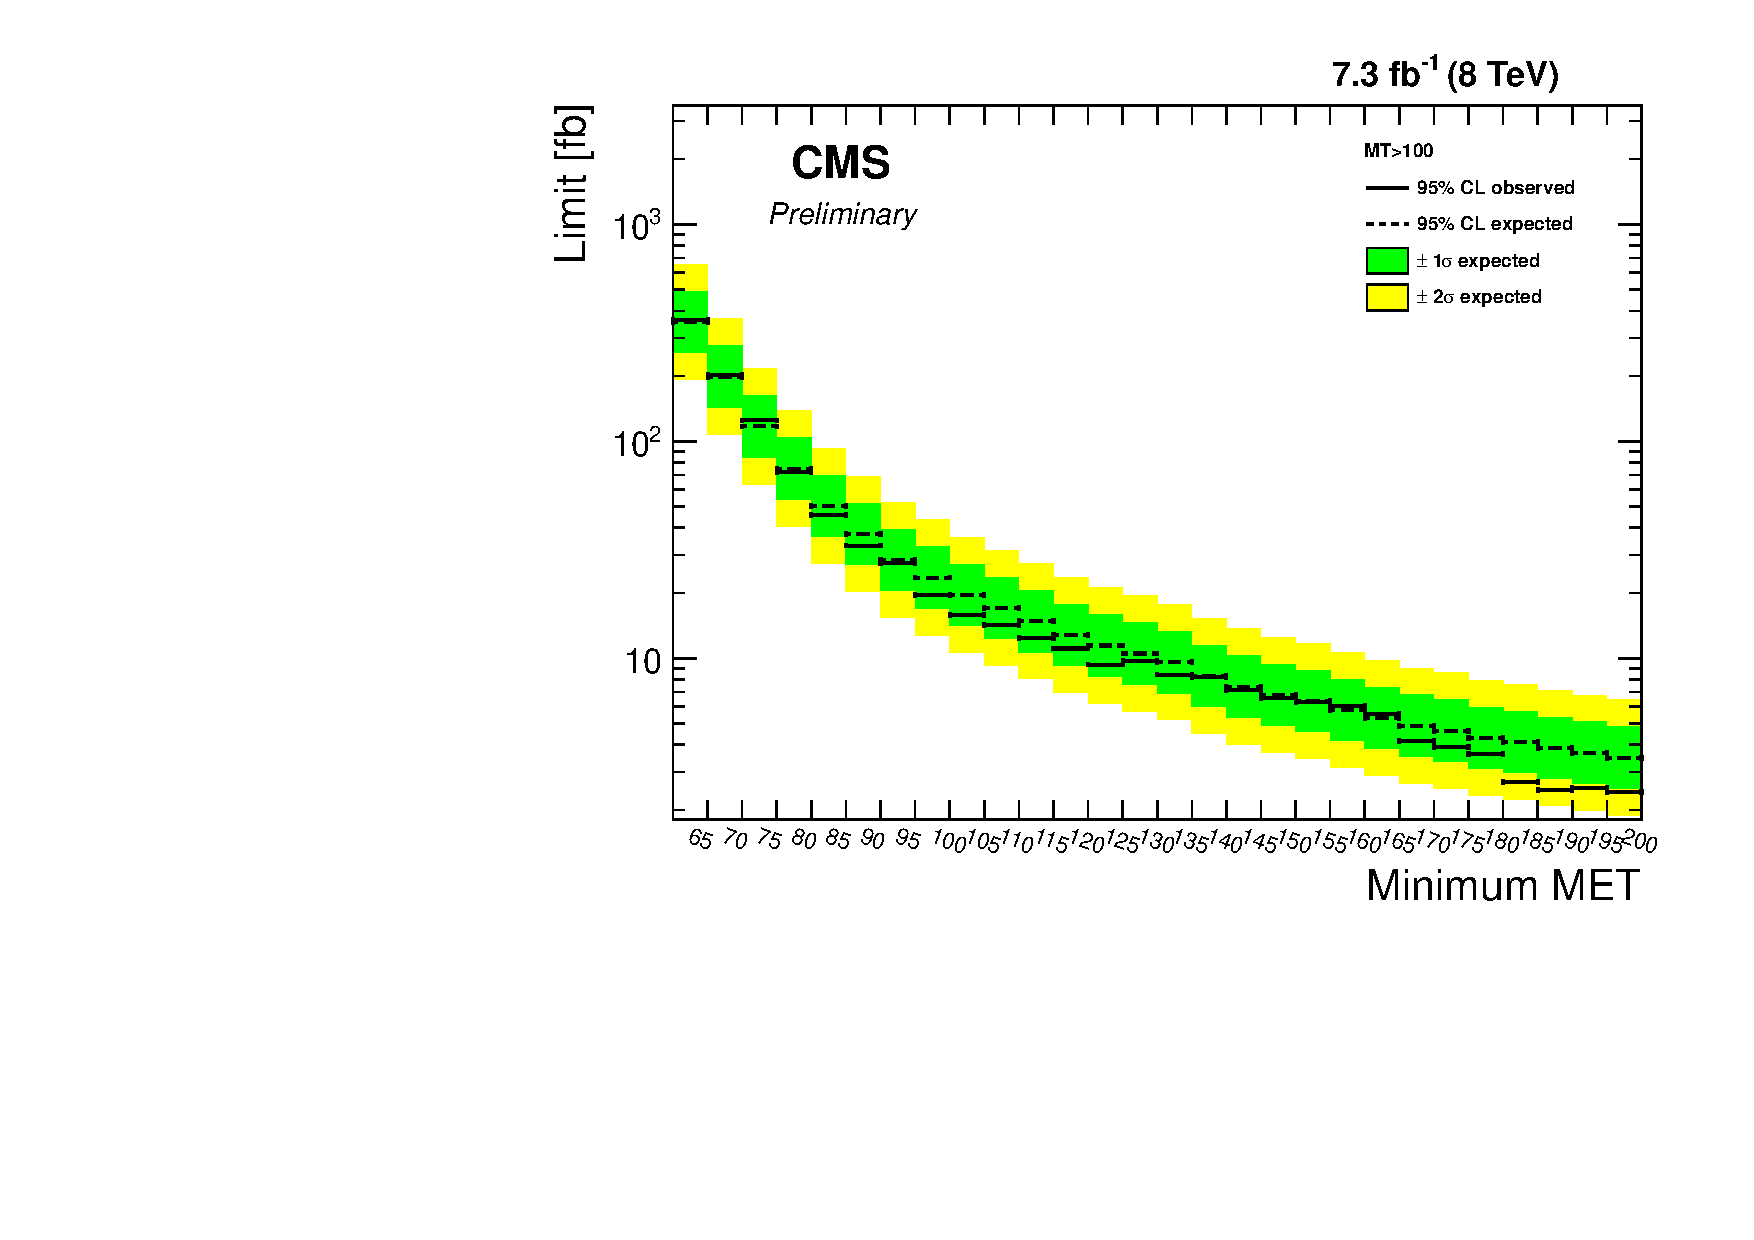
\includegraphics[scale=0.4]{Unblinding/ModelIndep/LimitPlotVsMET_MT100.pdf}}
\caption{ The expected (a) and observed (b) 95$\%$ CL upper limit on $\sigma \times BR\times A\times\epsilon$ for different $M_{T}$ and \met thresholds and (c) for $M_{T}> 100$ GeV as function of the \met threshold.}
\label{fig:limit_MI}      
\end{figure}    


\subsection{Model-specific limits}

   %%-------Higgs EXO limit 
   The yields for supersymmetric decays of the Higgs boson ($h\to \PXXSG\PSGczDo,\PSGczDo\to\PXXSG\gamma$) are acquired through imposing the model-specific selection described in Section~\ref{sec:event_selection}. The yields for this selection are shown in Table~\ref{tab:exoh}. The 95$\%$ CL upper limits on the $\sigma \times$ branching ratio(BR) and ($\sigma \times BR )/ \sigma_{SM}$, where $\sigma_{SM}$ is the cross section for the standard model Higgs boson, are evaluated for different mass values of \PSGczDo ranging from 65\GeV to 120\GeV and are shown in Fig.~\ref{fig:limit_higgs}.   
                       
\begin{table}[H]
\centering
\begin{tabular}{|c|c|}
\hline
Process 						& 			Estimate \\ \hline
$\gamma +$ jets                         	& 			179 $\pm$ 28 \\
${\rm jet}\rightarrow \gamma$		& 			269 $\pm$ 94 \\
${\rm e} \rightarrow \gamma$		&			355 $\pm$ 28 \\
$W(\to \ell\nu)+\gamma $			&			154 $\pm$ 15 \\
$Z( \to \nu \bar{\nu} )+\gamma$  	&  			182 $\pm$ 13 \\
Other                                    		&  			91 $\pm$  10 \\ \hline
Total background                       		&   			1232 $\pm$ 188 \\ \hline
Data                                   		&  			1296  \\ \hline \hline
$M_{\PSGczDo}$ = 65~\GeV 		& 			653.0 $\pm$ 77 \\
$M_{\PSGczDo}$ = 95~\GeV 		& 			1158.1  $\pm$ 137\\
$M_{\PSGczDo}$ = 120~\GeV 		& 			2935.0 $\pm$ 349 \\ \hline
\end{tabular}

\caption{Expected (SM background) and observed event yields after the selection optimized for the supersymmetric decay of the Higgs boson ($h\to\PXXSG\PSGczDo,\PSGczDo\to\PXXSG\gamma$) and the signal predictions  correspond to BR($H \rightarrow $invisible + $\gamma$) =100\%.}

\label{tab:exoh}

\end{table}


\begin{figure}[H]
\centering
{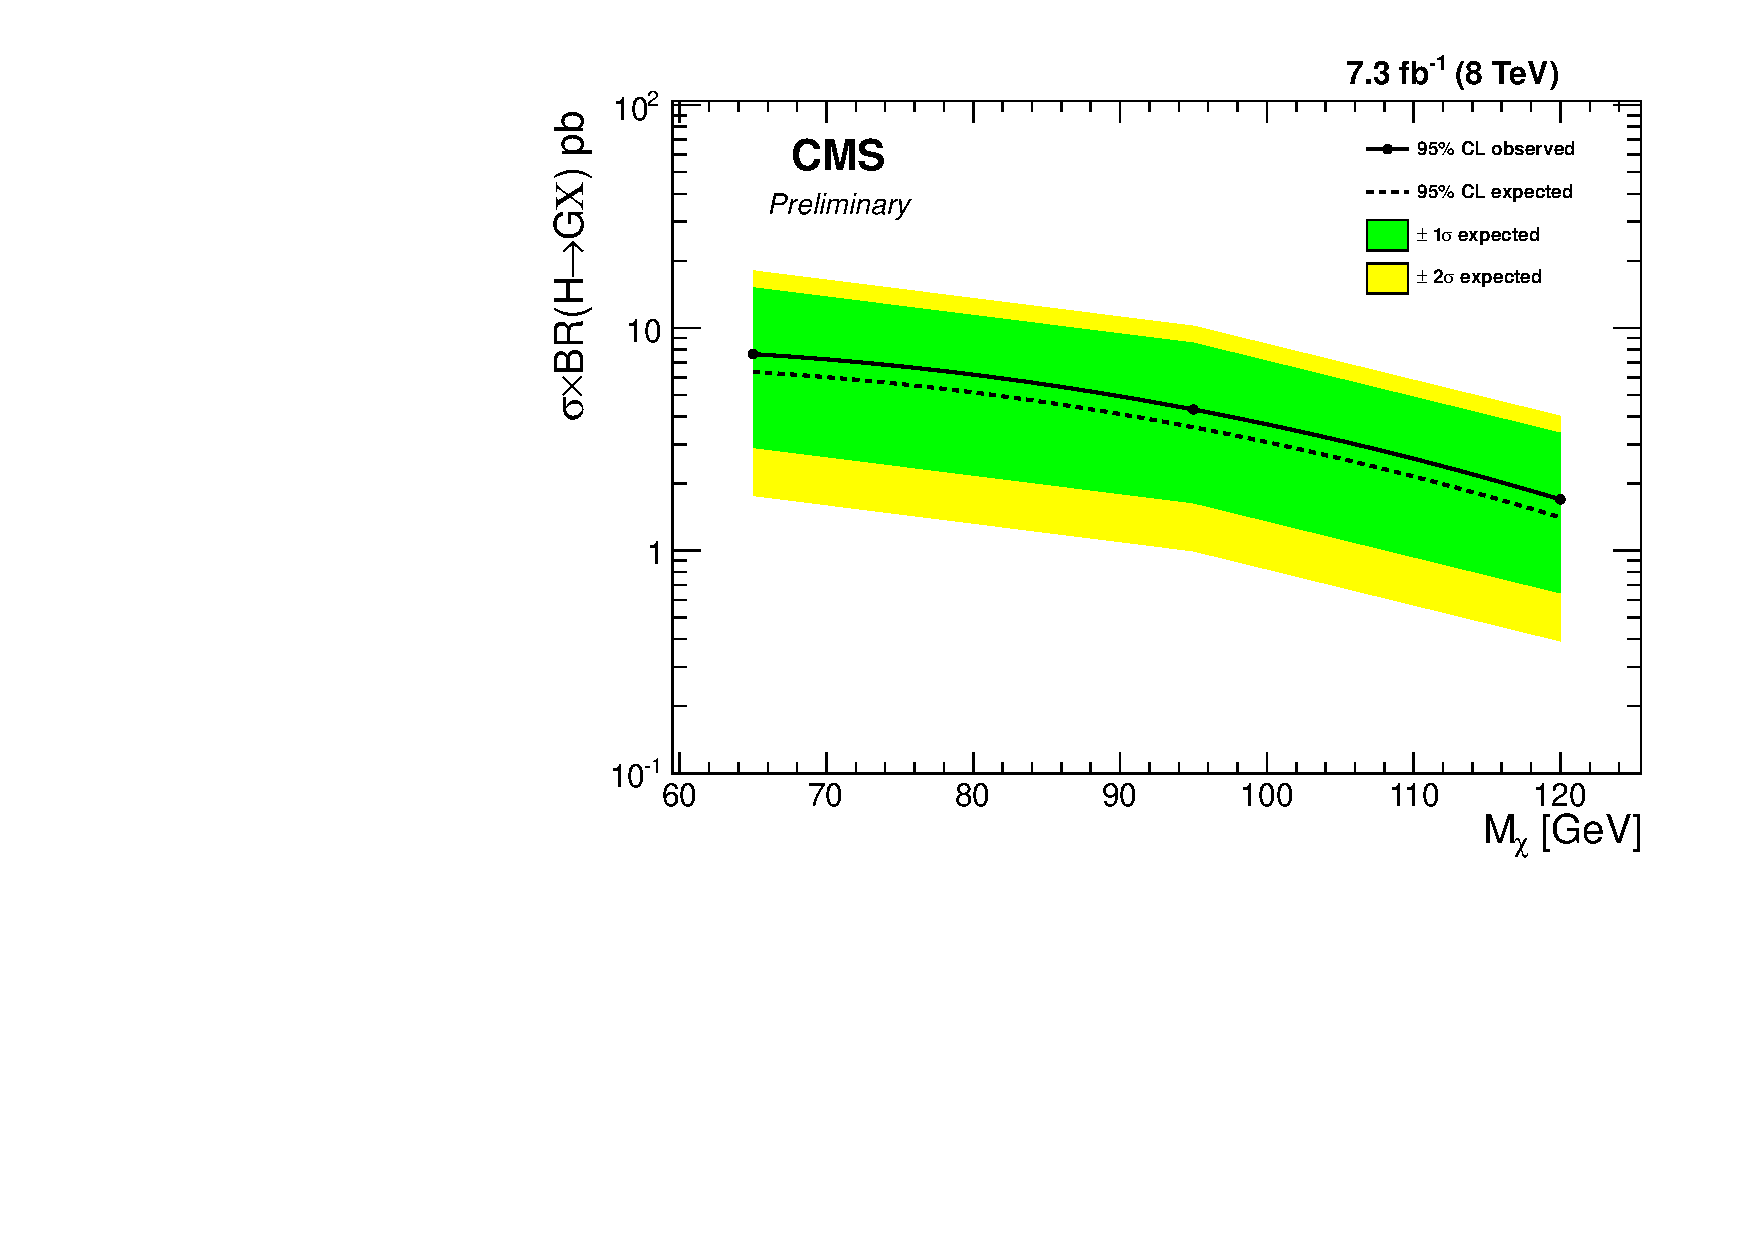
\includegraphics[width=0.45\textwidth]{PAS_Plots2/limit_xsec.pdf}}
{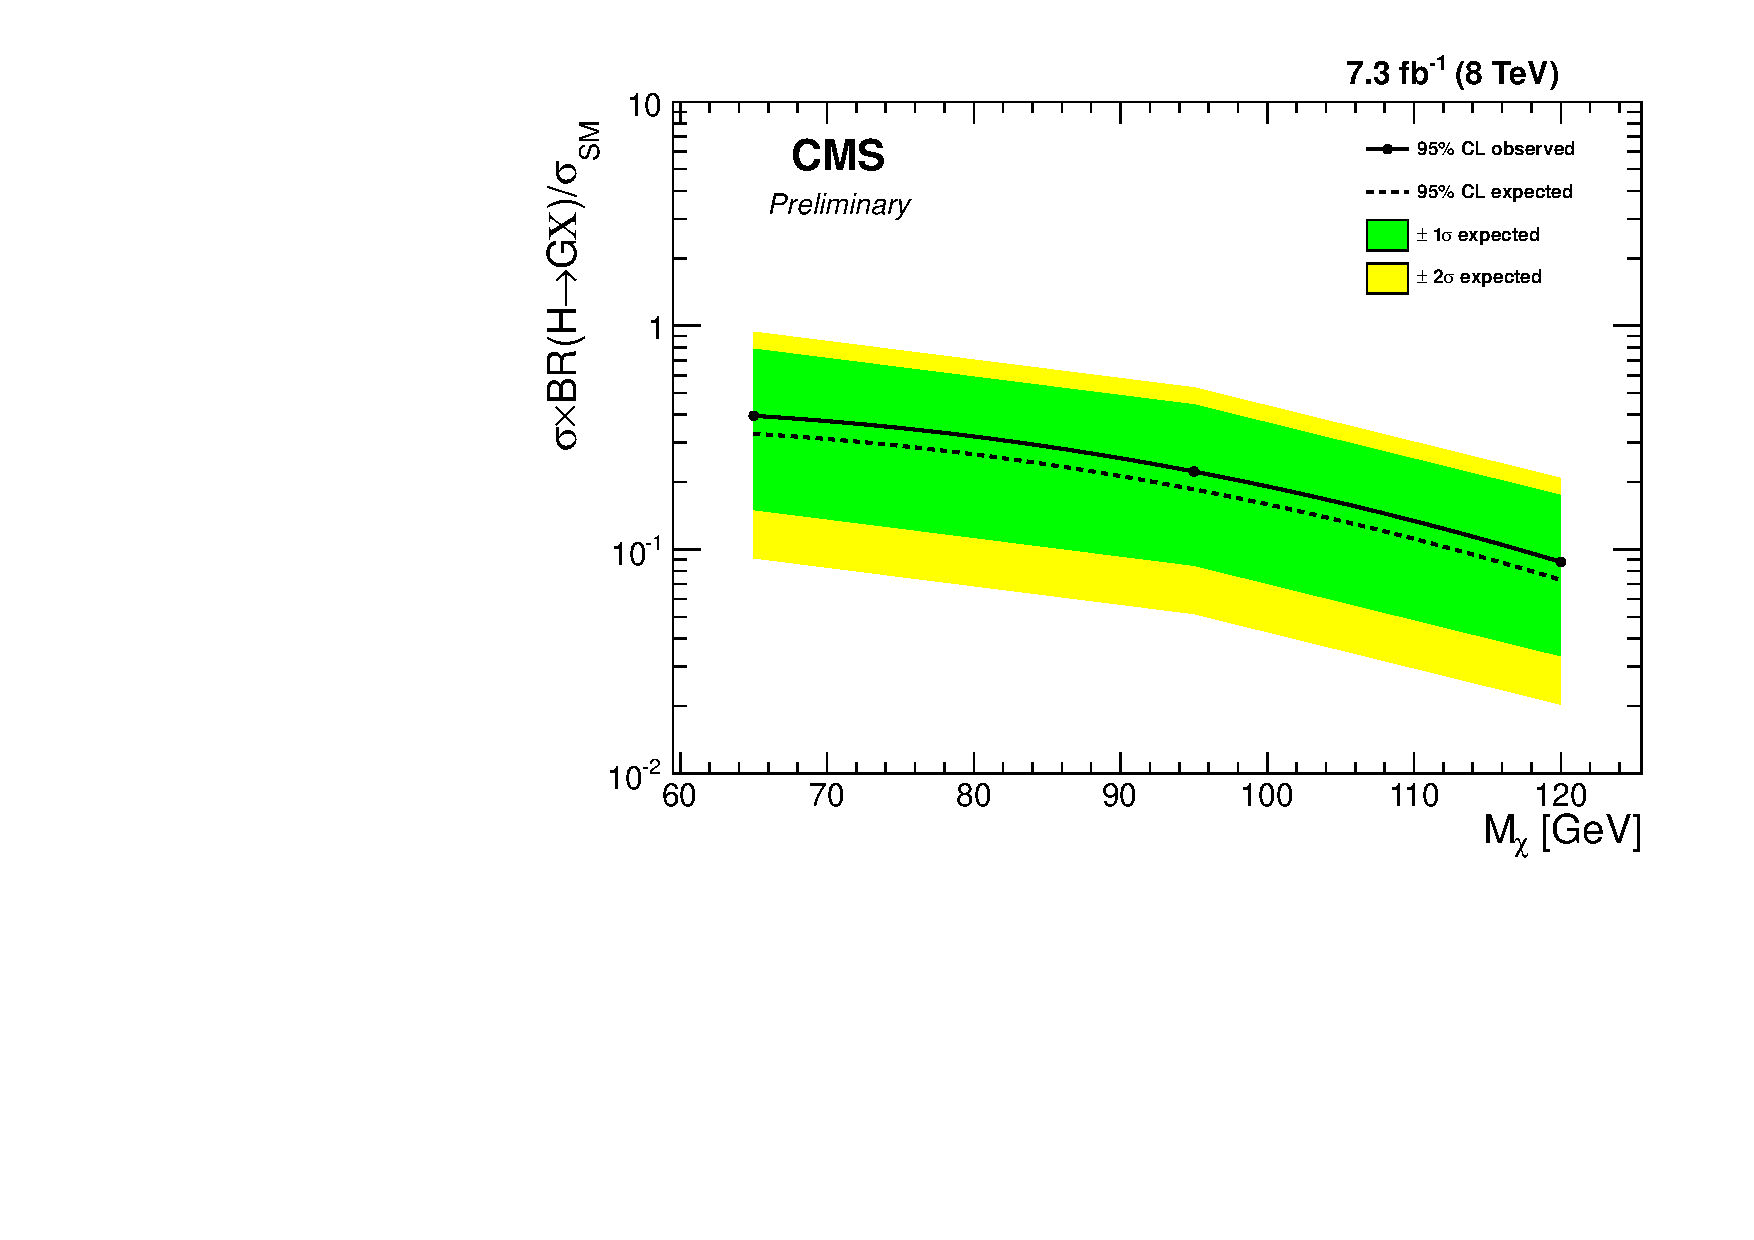
\includegraphics[width=0.45\textwidth]{PAS_Plots2/limit_ratio.pdf}}
%{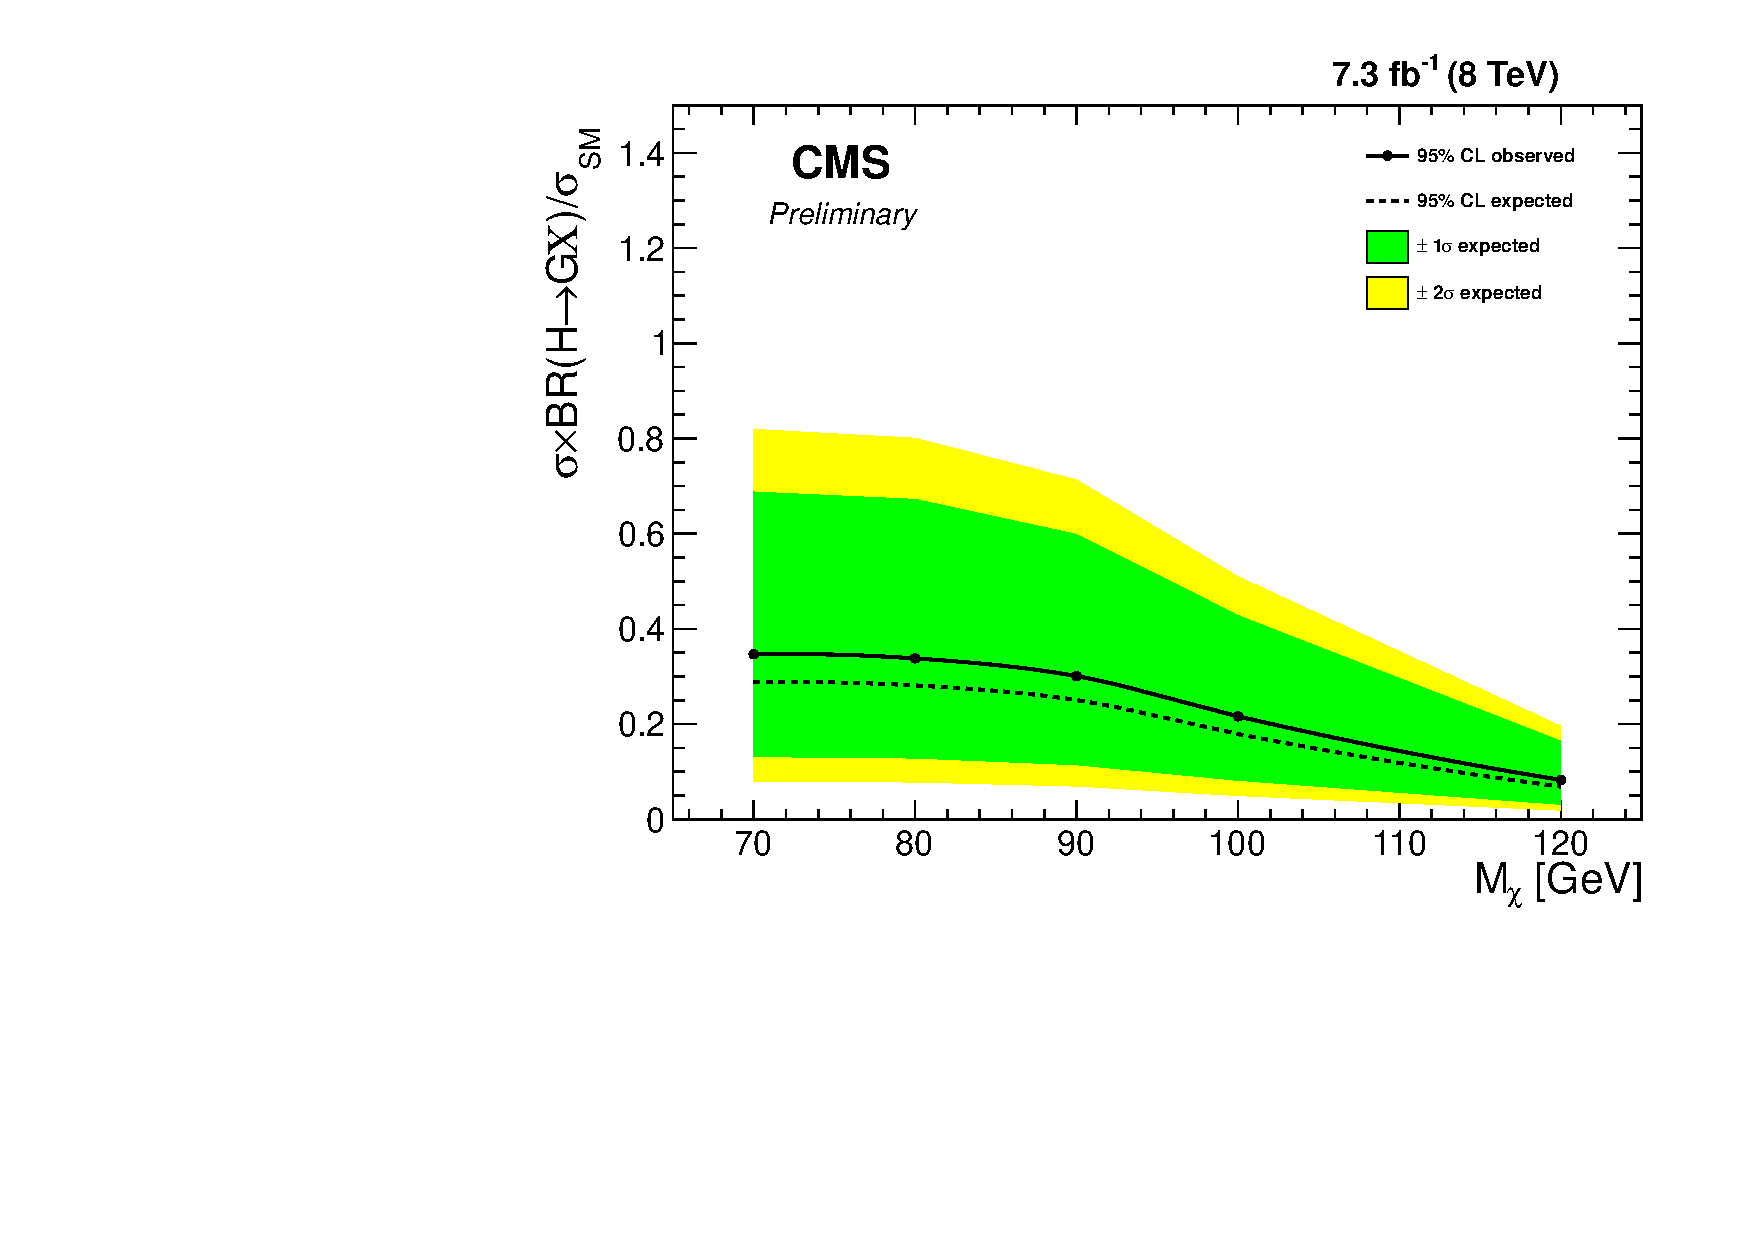
\includegraphics[scale=0.4]{Unblinding/Susy/ratio.pdf}}
%{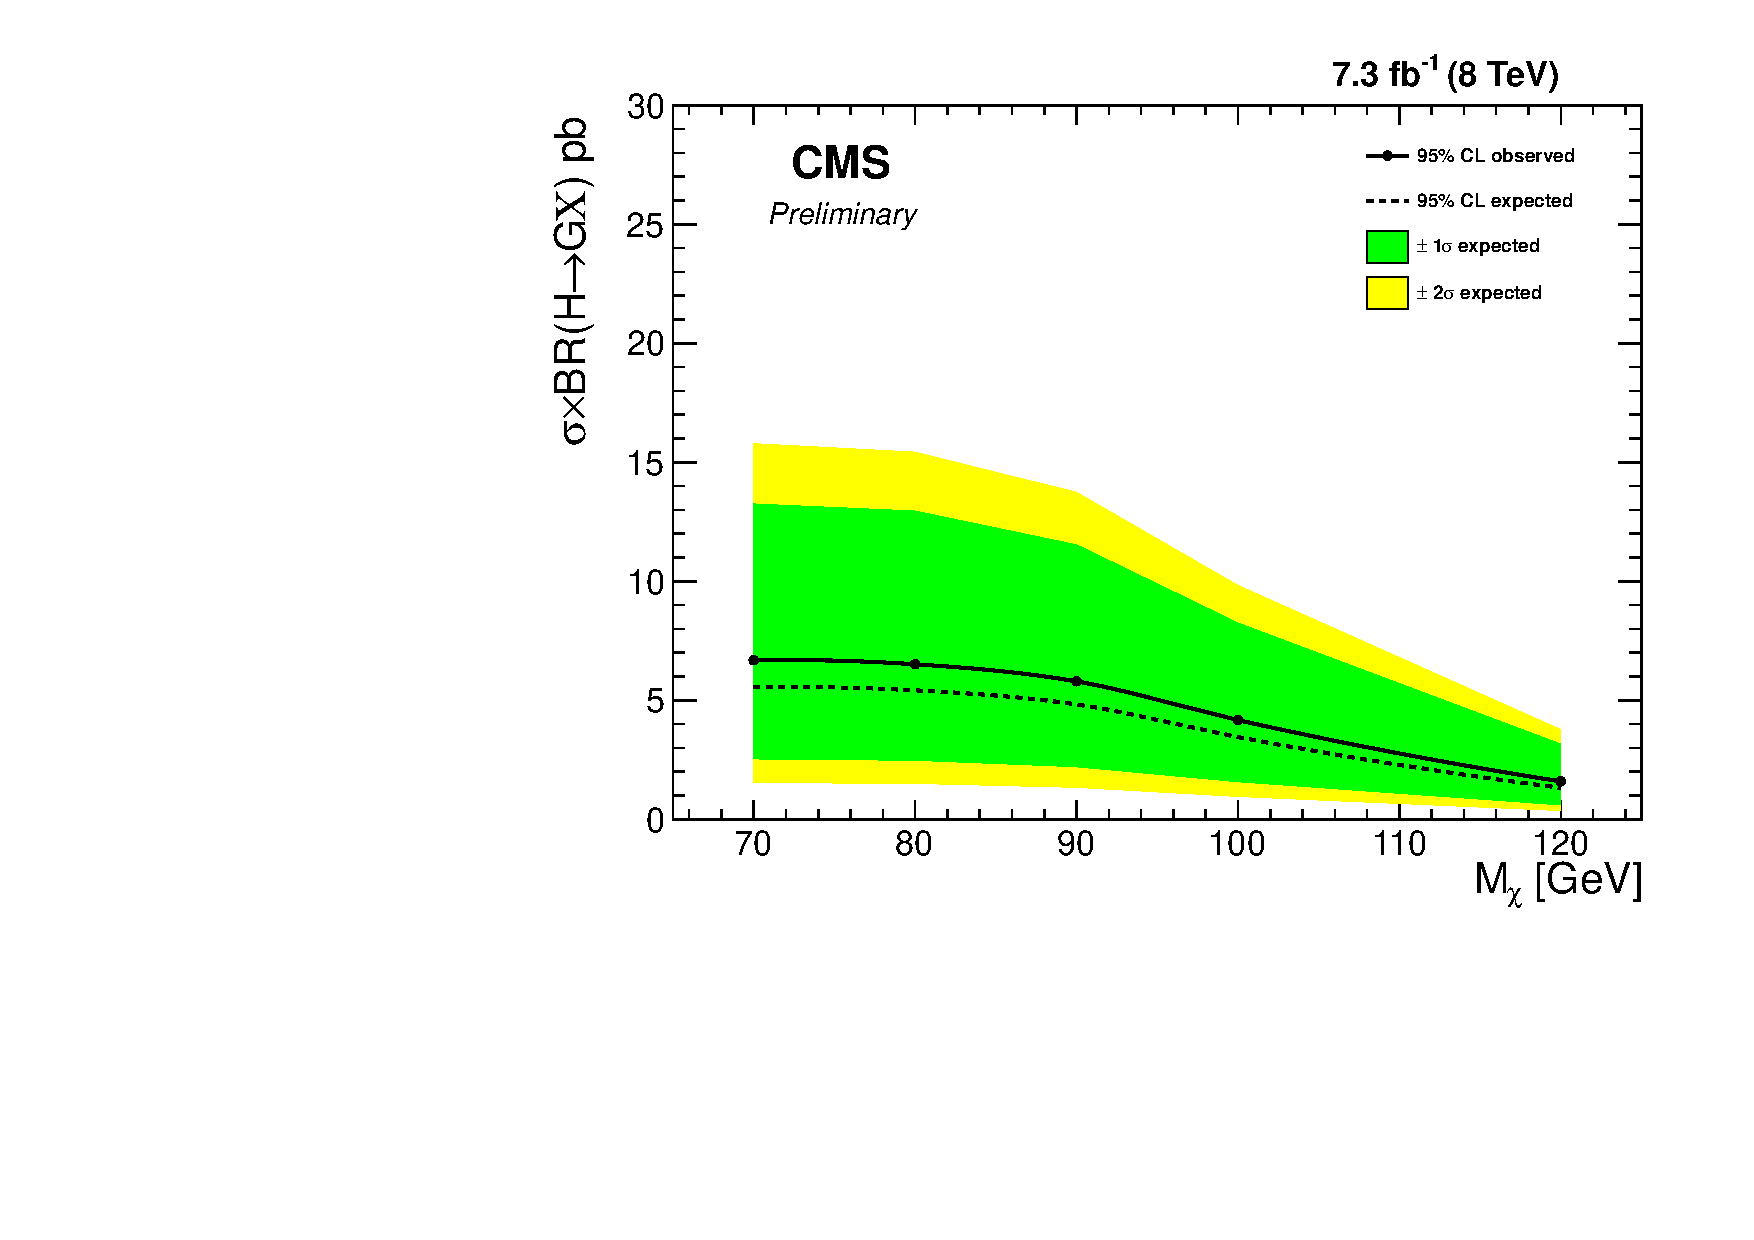
\includegraphics[scale=0.4]{Unblinding/Susy/xsec.pdf}}
\caption{ Expected and observed 95\% CL upper limits on (a) $\sigma \times BR$ and (b) the ratio of this product over the SM Higgs production cross section as a function of different $M_{\PSGczDo}$ values. The uncertainty on the expected limit at 1$\sigma$ and 2$\sigma$ levels are shown as green and yellow bands, respectively. }
\label{fig:limit_higgs}    
\end{figure}


  %%-----DM Limits and plots
%   In the case of dark matter production, lower bounds are evaluated for the cut-off scale $\Lambda$ and then converted to limits on the $\chi$-nucleon cross section using the relation in Eqn.~\ref{eq:dmXS} under the EFT approximation.

 %%-----DM Table Vector
%\begin{table}[H]                                                                  
%\center    
%{ 
%\begin{tabular}{|c|c|c|c|}                                                             
%\hline
% $M_{\chi}$ (\GeV) & $\Lambda$ (\GeV) & $\sigma$ (fb) & $\chi$-nucleon ($\cm^{2}$) \\       
%\hline
% 1    &  ()  &  () & ()  \\
% 10   &  () &  () &  () \\
% 100  &  () & ()  &  () \\
% 200  &  () & ()  &  () \\
% 500  &  () & ()  &  () \\
% 1000 &  () & ()  &  () \\
%\hline
%\end{tabular}  
%\caption{The observed (expected) 90$\%$ CL upper limit on production cross section ($\sigma$), 90$\%$ CL lower bounds on scale $\Lambda$ and $90\%$ CL upper limits on $\chi$-nucleon cross section within the EFT framework for vector operator, for different $M_{\chi}$ masses.}                     
%\label{table:Vdm}                                                                 
%}
%\end{table}

 %%-----DM Table Axial-Vector
%\begin{table}[H]                                                                  
%\center    
%{ 
%\begin{tabular}{|c|c|c|c|}                                                             
%\hline
% $M_{\chi}$ (\GeV) & $\Lambda$ (\GeV) & $\sigma$ (fb) & $\chi$-nucleon ($\cm^{2}$) \\       
%\hline
% 1    & ()  & ()  & ()  \\
% 10   & ()  & ()  & ()  \\
% 100  & ()  & ()  & ()  \\
% 200  & ()  & ()  & ()  \\
% 500  & ()  & ()  & ()  \\
% 1000 & ()  & ()  & ()  \\
%\hline
%\end{tabular} 
%\caption{The observed (expected) 90$\%$ CL upper limit on production cross section ($\sigma$), 90$\%$ CL lower bounds on scale $\Lambda$ and $90\%$ CL upper limits on $\chi$-nucleon cross section within the EFT framework for axial-vector operator, for different $M_{\chi}$ masses.} 
%\label{table:AVdm}                                                                 
%}
%\end{table}

 %%------- Limit ploto for DM
%\begin{figure}[H]
%\centering
%{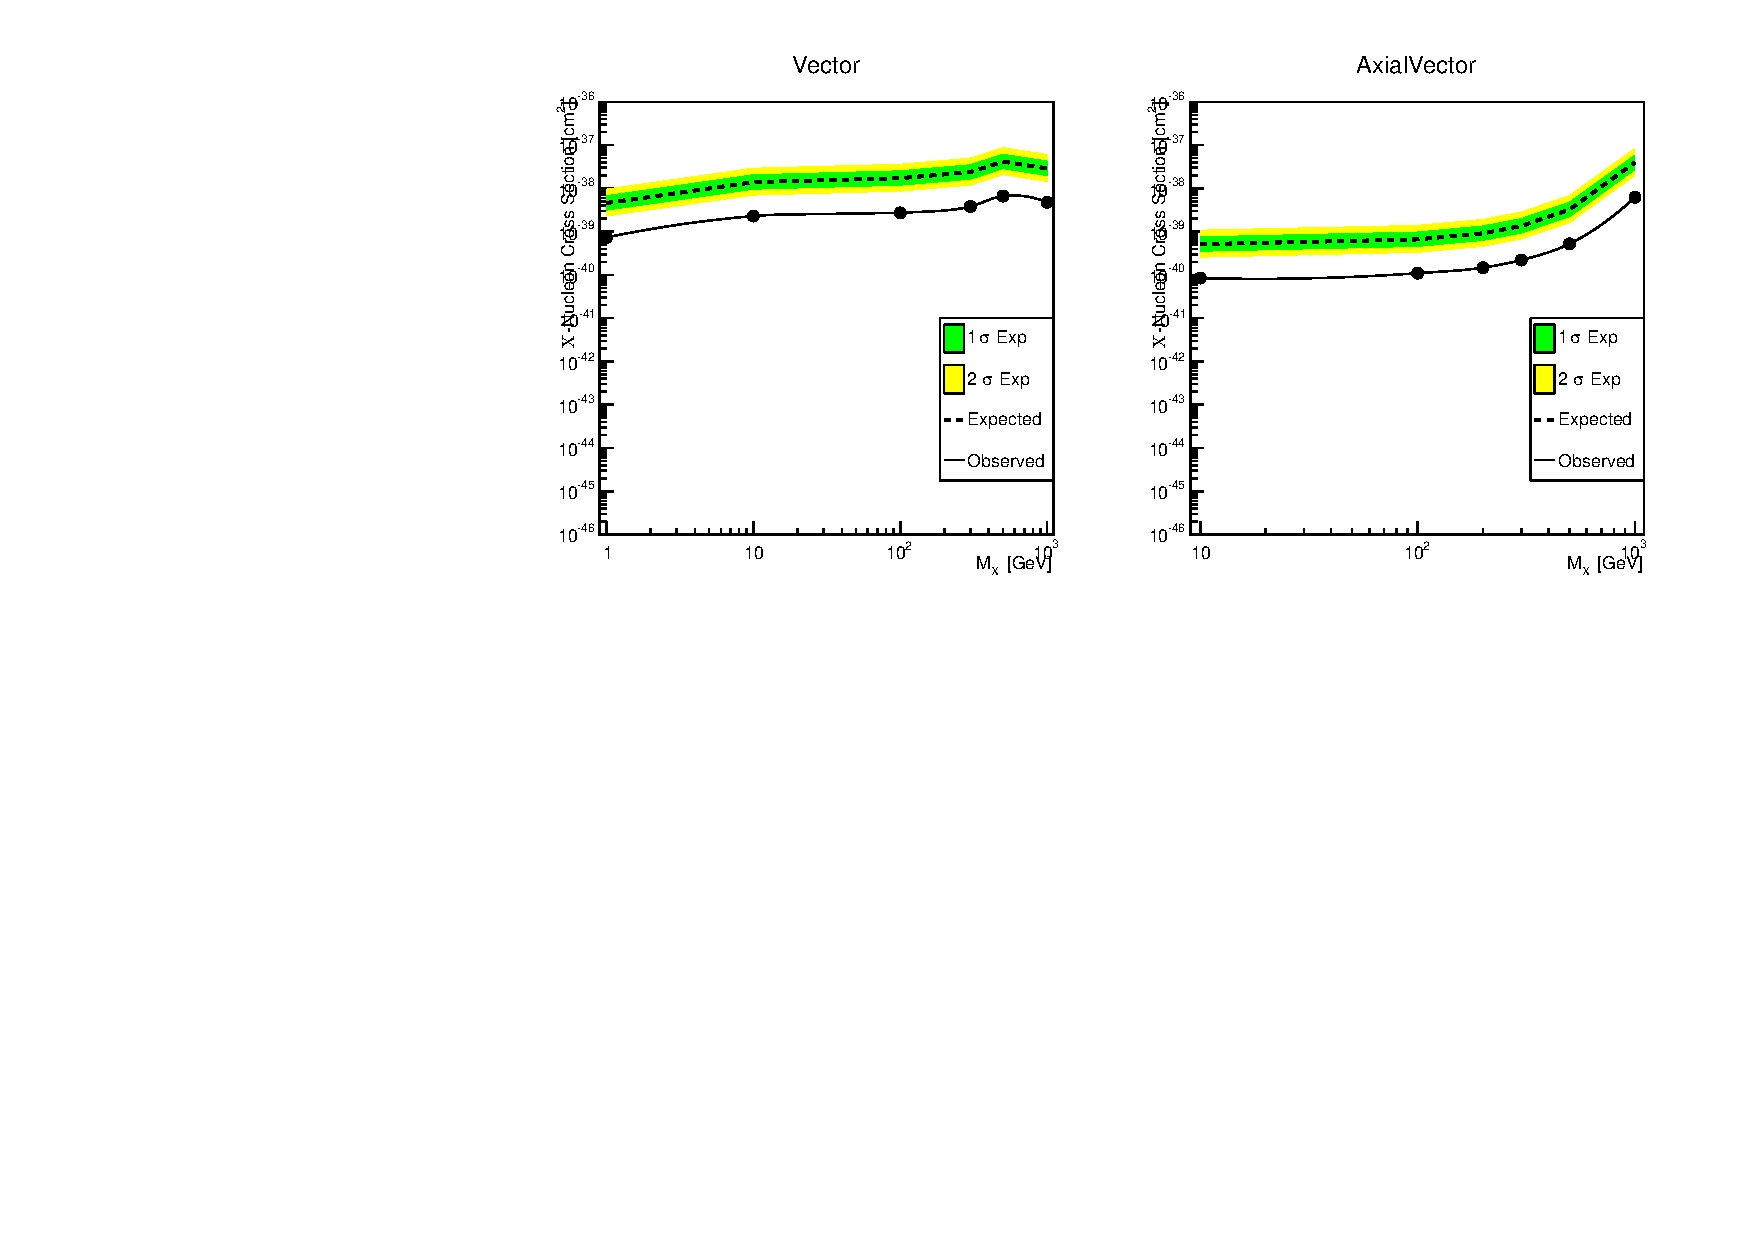
\includegraphics[scale=0.7]{figures/LowEt_DM.pdf}}
%%{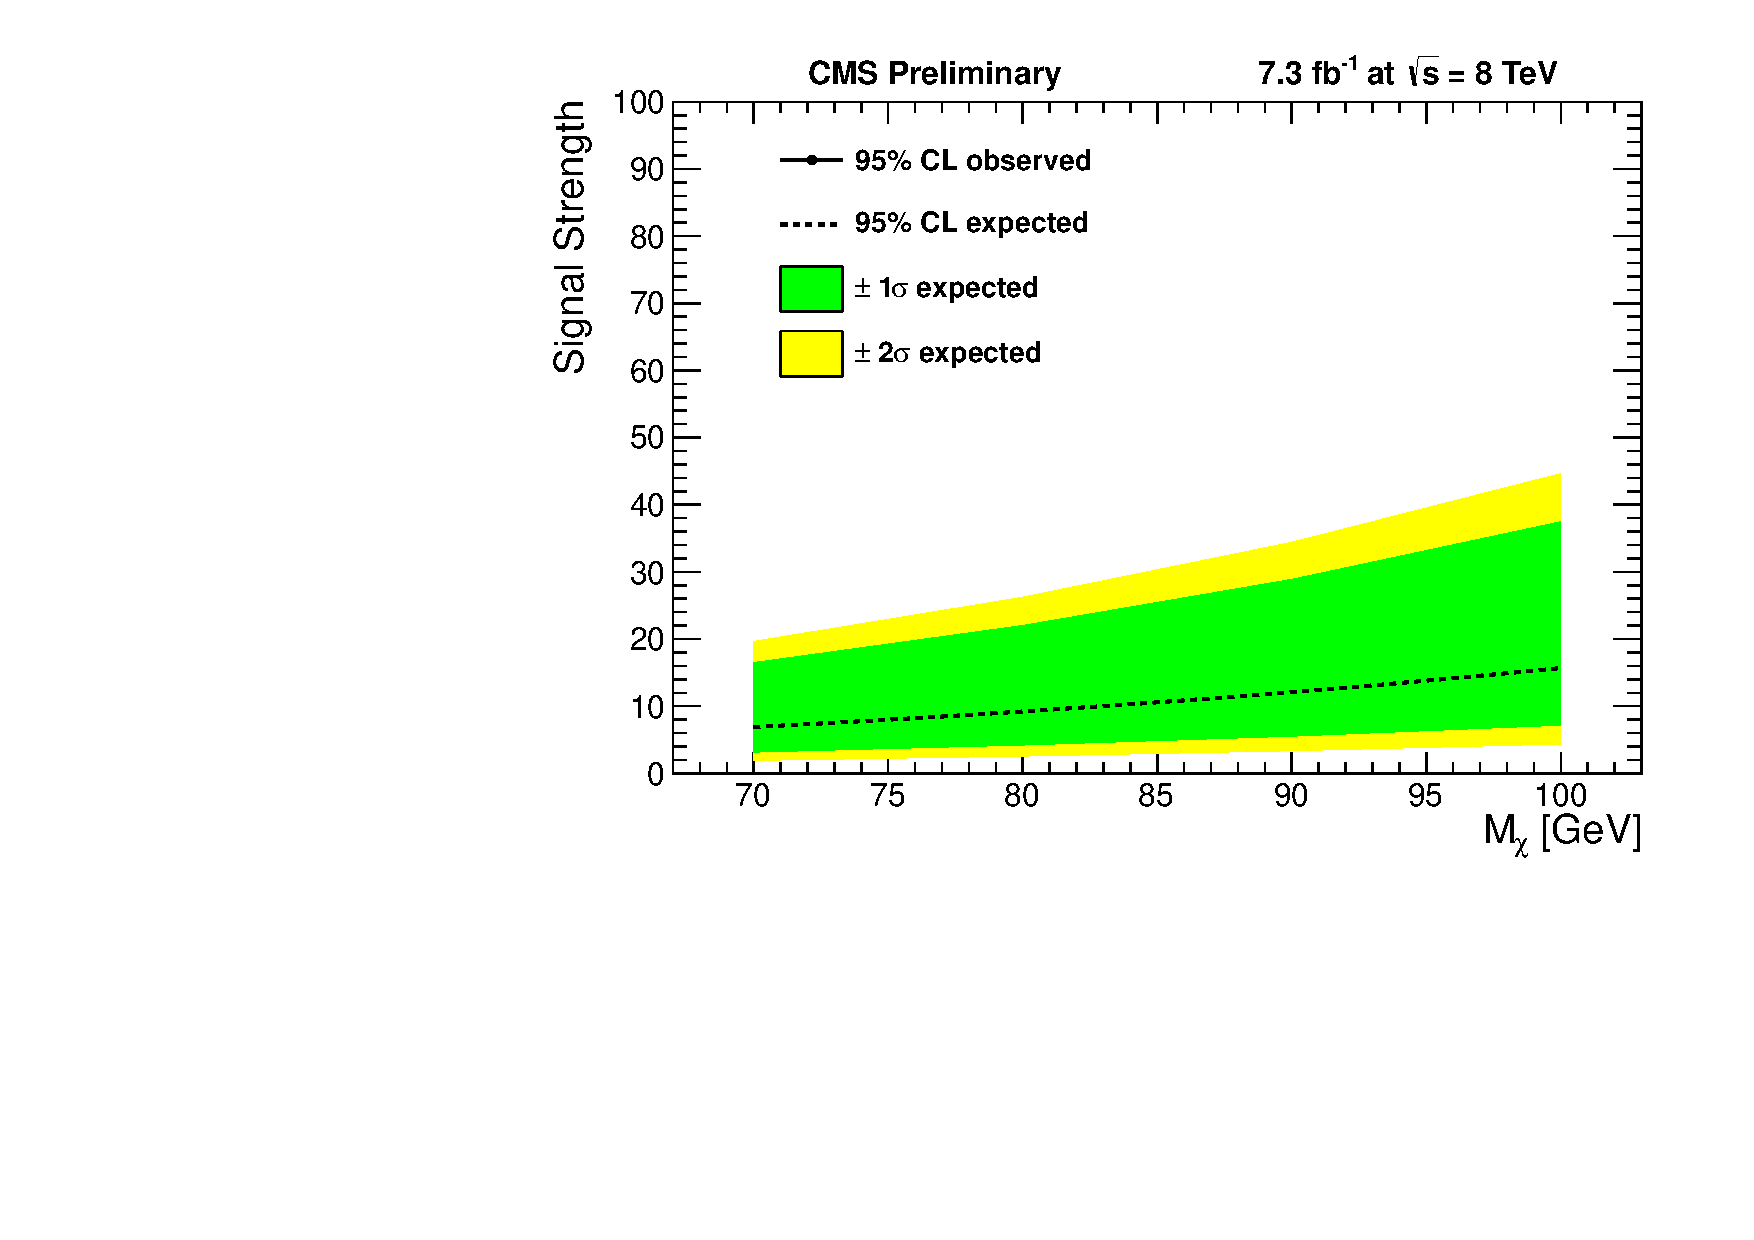
\includegraphics[scale=0.45]{figures/exoh_limit.pdf}}
%\caption{ The 90$\%$ CL upper limits on $\chi$-nucleon cross section for (a) vector and (b) axial-vector interaction for $\gamma\chi\chi$ production under the EFT assumption. The direct detection results from different experiments~\cite{CDMS2,XENON100,PICASSO,COUPP,COGENT,CDMSLITE,LUX} are also shown for comparison. The limits from high \pt searches at $\sqrt{s}= 8$ TeV in the monophoton final state are also shown from the CMS~\cite{CMS:2014mea} and ATLAS~\cite{ATLASmono} experiments. }
%\label{fig:DMlimits}
%\end{figure}

%  Tables~\ref{table:Vdm} and \ref{table:AVdm} show the $90\%$ CL lower bound on $\Lambda$ and corresponding upper limits on the $\chi$-nucleon cross section for different $M_{\chi}$ values. These limits are evaluated for spin-independent and spin-dependent operators. Fig.~\ref{fig:DMlimits} shows these limits as a function of $M_{\chi}$ and compares these results with other direct detection experiments~\cite{CDMS2,XENON100,PICASSO,COUPP,COGENT,CDMSLITE,LUX}. The results from previous high \pt ( \pt $> 125$ GeV) searches at the LHC are also shown~\cite{CMS:2014mea,ATLASmono}.   


























